\documentclass[12pt,a4paper]{report}

\usepackage{styles/dolgozat}
\usepackage{listings}
\usepackage{styles/python}
\usepackage{hyperref}

\parskip=20pt

\begin{document}

\pagestyle{empty} %a címlapon ne legyen semmi=empty, azaz nincs fejléc és lábléc

% A Miskolci Egyetem címere
{\large
\begin{center}
\vglue 1truecm
\textbf{\huge\textsc{Szakdolgozat}}\\
\vglue 1truecm

\includegraphics[width=4.8truecm, height=4truecm]{images/me_logo.png}\\
\textbf{\textsc{Miskolci Egyetem}}
\end{center}}

\vglue 1.5truecm %függõleges helykihagyás

% A szakdolgozat címe, akár több sorban is
{\LARGE
\begin{center}
\textbf{Órarendgenerálási problémák megoldása hagyományos és genetikus algoritmusokkal}
\end{center}}

\vspace*{2.5truecm}
% A hallgató neve, évfolyam, szak(ok), a konzulens(ek) neve
{\large
\begin{center}
\begin{tabular}{c}
\textbf{Készítette:}\\
Molnárfi Brendon\\
Programtervező informatikus
\end{tabular}
\end{center}
\begin{center}
\begin{tabular}{c}
\textbf{Témavezető:}\\
Piller Imre
\end{tabular}
\end{center}}
\vfill
% Keltezés: Hely, év
{\large
\begin{center}
\textbf{\textsc{Miskolc, 2021}}
\end{center}}

\newpage

%Feladatkiiras
\pagestyle{empty}
\begin{flushleft}
\textsc{\bfseries Miskolci Egyetem}\\
Gépészmérnöki és Informatikai Kar\\
Alkalmazott Matematikai Intézeti Tanszék\hspace*{4cm}\hfil \textbf{Szám:}
\end{flushleft}
\vskip 0.5cm
\begin{center}
\large\textsc{\bfseries Szakdolgozat Feladat}
\end{center}
\vskip 0.5cm
Molnárfi Brendon (GAX11M) programtervező informatikus jelölt részére.\newline

\noindent\textbf{A szakdolgozat tárgyköre:} órarend, optimalizálás, genetikus algoritmus\newline

\noindent\textbf{A szakdolgozat címe:} Órarendgenerálási problémák megoldása hagyományos és\newline genetikus algoritmusokkal\newline

\noindent\textbf{A feladat részletezése:}

\medskip

\emph{Órarendek tervezésére jellemzően az oktatásban szokott szükség lenni. A dolgozat azt vizsgálja, hogy különböző komplexitású problémákat milyen algoritmussal, és milyen hatékonysággal lehet megoldani.}

\medskip

\emph{A dolgozat legelőször sorra veszi a készen elérhető megoldási módszereket, a hozzájuk készített szoftvereket. Saját munka keretében bevezeti az órarendtervezési problémák absztrakt modelljeit, majd implementálja is a megoldásokat, sorrendben az egymásra épülő részfeladatok kapcsán, lépésről lépésre jutva el a minden tényezőt számontartó, és minden azokkal kapcsolatos feltételnek eleget tevő órarendig. A dolgozatban a genetikus algoritmus alkalmazása is fontos szerepet kap.}

\medskip

\emph{Az egyes részfeladatokat megoldó hagyományos algoritmusok, illetve genetikus algoritmus Python programozási nyelven készültek. A végén előállt órarendek táblázatos formában, grafikusan is megtekinthetők.}

\vfill

\noindent\textbf{Témavezető:} Piller Imre (egyetemi tanársegéd) \newline

% \noindent\textbf{Konzulens(ek):} (akkor kötelezõ, ha a témavezetõ nem valamelyik matematikai tanszékrõl való; de persze lehet egyébként is)\newline

\noindent\textbf{A feladat kiadásának ideje:}\newline

%\noindent\textbf{A feladat beadásának határideje:}

\vskip 2cm

\hbox to \hsize{\hfil{\hbox to 6cm {\dotfill}\hbox to 1cm{}}}

\hbox to \hsize{\hfil\hbox to 3cm {szakfelelős}\hbox to 2cm{}}

\newpage

\vspace*{1cm}  
\begin{center}
\large\textsc{\bfseries Eredetiségi Nyilatkozat}
\end{center}
\vspace*{2cm}  

Alulírott \textbf{Molnárfi Brendon}; Neptun kód: \texttt{GAX11M} a Miskolci Egyetem Gépészmérnöki és Informatikai Karának végzős Programtervező informatikus szakos hallgatója ezennel büntetőjogi és fegyelmi felelősségem tudatában nyilatkozom és aláírásommal igazolom, hogy \textit{Órarendgenerálási problémák megoldása hagyományos és genetikus algoritmusokkal} című szakdolgozatom saját, önálló munkám; az abban hivatkozott szakirodalom
felhasználása a forráskezelés szabályai szerint történt.\\

Tudomásul veszem, hogy szakdolgozat esetén plágiumnak számít:
\begin{itemize}
\item szószerinti idézet közlése idézőjel és hivatkozás megjelölése nélkül;
\item tartalmi idézet hivatkozás megjelölése nélkül;
\item más publikált gondolatainak saját gondolatként való feltüntetése.
\end{itemize}

Alulírott kijelentem, hogy a plágium fogalmát megismertem, és tudomásul veszem, hogy
plágium esetén szakdolgozatom visszautasításra kerül.

\vspace*{3cm}

\noindent Miskolc, \hbox to 2cm{\dotfill} .év \hbox to 2cm{\dotfill} .hó \hbox to 2cm{\dotfill} .nap

\vspace*{3cm}

\hspace*{8cm}\begin{tabular}{c}
\hbox to 6cm{\dotfill}\\
Hallgató
\end{tabular}

\newpage

\noindent 1.

\begin{tabular}{cl}
&szükséges (módosítás külön lapon) \\
A szakdolgozat feladat módosítása& \\
& nem szükséges\\
&\\
\hbox to 4cm{\dotfill}&\multicolumn{1}{c}{\hbox to 5cm{\dotfill}}\\
dátum& \multicolumn{1}{c}{témavezető(k)}
\end{tabular}
\vskip1.5mm

\noindent 2. A feladat kidolgozását ellenőriztem:

\vskip1.5mm

\begin{tabular}{l@{\hspace*{4cm}}l}
témavezető (dátum, aláírás):& konzulens (dátum, aláírás):\\
\dotfill&\dotfill\\
\dotfill&\dotfill\\
\dotfill&\dotfill
\end{tabular}

\vskip1.5mm

\noindent 3. A szakdolgozat beadható:

\vskip1.5mm

\begin{tabular}{@{\hspace*{1.3cm}}c@{\hspace*{2.1cm}}c}
\hbox to 4cm{\dotfill}&\multicolumn{1}{c}{\hbox to 5cm{\dotfill}}\\
dátum& \multicolumn{1}{c}{témavezető(k)}
\end{tabular}

\vskip1.5mm

\noindent 4.
\begin{tabular}[t]{@{}l@{\hspace*{1mm}}l@{\hspace*{1mm}}l@{}}
A szakdolgozat& \hbox to 3.5cm{\dotfill} &szövegoldalt\\
              & \hbox to 3.5cm{\dotfill} &program protokollt (listát, felhasználói leírást)\\
              &\hbox to 3.5cm{\dotfill}   &elektronikus adathordozót (részletezve)\\
              &\hbox to 3.5cm{\dotfill} & \\
              &\hbox to 3.5cm{\dotfill} &egyéb mellékletet (részletezve)\\
              &\hbox to 3.5cm{\dotfill} &\\
\end{tabular}
\newline tartalmaz.

\vskip1.5mm

\begin{tabular}{@{\hspace*{1.3cm}}c@{\hspace*{2.1cm}}c}
\hbox to 4cm{\dotfill}&\multicolumn{1}{c}{\hbox to 5cm{\dotfill}}\\
dátum& \multicolumn{1}{c}{témavezető(k)}
\end{tabular}

\noindent 5.

\begin{tabular}{ll}
&bocsátható\\
A szakdolgozat bírálatra& \\
& nem bocsátható\\
\end{tabular}

\vskip1.5mm

\noindent A bíráló neve: \hbox to 8cm{\dotfill}

\vskip4mm

\begin{tabular}{@{\hspace*{1.3cm}}c@{\hspace*{2.1cm}}c}
\hbox to 4cm{\dotfill}&\multicolumn{1}{c}{\hbox to 5cm{\dotfill}}\\
dátum& \multicolumn{1}{c}{szakfelelős}
\end{tabular}

\noindent 6.
\begin{tabular}[t]{@{}l@{\hspace*{1mm}}l@{\hspace*{1mm}}l@{}}
A szakdolgozat osztályzata& &\\
&a témavezető javaslata:& \hbox to 3cm{\dotfill}\\
&a bíráló javaslata:& \hbox to 3cm{\dotfill}\\
&a szakdolgozat végleges eredménye:& \hbox to 3cm{\dotfill}
\end{tabular}

\vspace*{4mm}

\noindent Miskolc, \hbox to 4.5cm{\dotfill} \hspace*{2.5cm}
\begin{tabular}[t]{cc}
\hbox to 6cm{\dotfill}\\
a Záróvizsga Bizottság Elnöke
\end{tabular}

\newpage

\cleardoublepage
\pagenumbering{gobble}

\tableofcontents

\noindent \textbf{Summary} \hfill{\textbf{50}}

\noindent \textbf{Irodalomjegyzék} \hfill{\textbf{50}}

\noindent \textbf{Adathordozó használati útmutató} \hfill{\textbf{50}}

\cleardoublepage
\pagenumbering{arabic}

\newpage

\pagestyle{fancy}

\Chapter{Bevezetés}

Az iskolák és egyetemek a különböző osztályok, tanárok és tantermek órarendjének 
elkészítéséhez ma már számítógépes segítséget használnak, hagyományos algoritmusokat és a
mesterséges intelligencia egyik elterjedt eszközét, a genetikus algoritmust. Máskülönben 
nagyon időigényes, fáradtságos munka lenne összesen többszáz órarend ütközésmentes 
összehangolása, hiszen ugyanannak az osztálynak egy időben nem lehet több tanórája, egy tanár
sem tud két helyen egyszerre jelen lenni és egy tanteremben sem lehet két tanóra egy időben,
ott van továbbá a termek kapacitása, a tanárok heti óraszámai közti különbségek 
minimalizálása, az új osztályok képzésének szükségessége, pl. nyelvi vagy fakultációs órák 
miatt, és ez még nem minden. Munkám során olyan algoritmusokat írok, melyeknek köszönhetően 
adathalmaz (osztályok, tanárok, tantermek, tantárgyak) megadása után ütközésmentes és minden
feltételnek eleget tevő órarendeket tudunk generálni, majd grafikus felhasználói felületet 
hozok létre fölötte, mégpedig webeset.

\newpage

\chapter{Előzetes tudnivalók}

\section{A genetikus algoritmus}

\subsection{Biológiai háttér}

Charles Darwin, angol biológus evolúcióelmélete paradigmaváltást hozott magával a biológiában. 
Lényege a fajok fennmaradásának, túlélésének genetikai háttére a Föld ökoszisztémáiban 
(életközösségeiben). Összetevői a szelekció, az öröklődés és a mutáció. A természetes 
szelekció értelmében a gyenge, vagyis kedvezőtlenebb, kevésbé optimális tulajdonságokkal 
rendelkező egyedeknek el kell pusztulniuk annak érdekében, hogy az adott faj populációja 
életképesebb legyen a következő generációkban. A kedvezőtlen gének továbbörökítése ezt
hátráltatná és mivel az állatvilágban táplálkozási hierarchia van, továbbá az éghajlati 
körülményekhez való alkalmazkodás is szerepet játszik a túlélésben, ebben az esetben félő 
lenne a populáció kihalása. A nőstények ösztönösen a kedvezőbb tulajdonságokkal rendelkező 
hímeket választják párosodásra, vagypedig egymás elleni csatában lejátsszák a hímek, ki 
juthasson hozzá a nőstényhez. Ez lehet nem halálos vagy halálos játszma is. Szintén kegyetlen 
világ figyelhető meg pl. a fókák esetében, ahol a győztes hím az összes nősténnyel párosodik, 
a vesztes pedig eggyel sem. Többnyire az erősebb egyedek örökítik így tovább a génjeiket, a
gyengébbek fokozatosan elhullanak a populációból, amely így generációról generációra erősebb,
életképesebb lesz. A mutáció szerepe is fontos, melynek eredménye hogy néha-néha egy egyed
valamely génje egyik szülőtől sem származó lesz, hanem egészen más lesz, következményként
nagymértékben különbözni fog mindkét szülőtől valamely tulajdonság kapcsán. Ez a jelenség is 
jó a populáció számára, mert csökkenti a belterjesség mértékét, a korai generációk folyamán
bekövetkező mutációk segíthetnek az adott ökoszisztémában hasznos, korábban nem jellemző
tulajdonságok térnyerésében, a későbbi mutációk már hamar elhalnak, nem játszanak szerepet. [1]

\subsection{Általánosságban a genetikus algoritmusról}

A genetikus algoritmusokat olyan diszkrét optimalizálási problémák megoldására alkalmazzuk,
amelyekre nem létezik általános eljárás, a probléma specifikussága, egyedisége következtében.
Túl sok az ismeretlen és a közöttük levő összefüggések is ismeretlenek, így a rendszernek 
"tanulnia kell" a probléma megoldása során, vagyis mesterséges intelligenciát kell 
használnunk. A genetikus algoritmus épp megfelel. Ahogyan az evolúció is lassú folyamat volt,
úgy az evolúciót modellező genetikus algoritmusok is lassúak, ahhoz képest hogy áramkörökről
beszélhetünk a háttérben, de nyilván nagyságrendekkel hamarabb kapunk eredményt, mintha emberi
intelligenciával dolgoznánk és amennyiben van megoldás, akkor azt egy megfelelően elkészített
genetikus algoritmus biztosan megtalálja. Mivel megelőzően nem lehetünk biztosak benne, hogy
egészen megfelelő paramétereket választottunk, az algoritmus többszöri lefuttatásával 
szerezhetünk bizonyosságot a megoldás optimális értékeit illetően. Ezenkívül van rá lehetőség,
hogy az algoritmus párhuzamosításával növeljük a gyorsaságot és csökkentsük a program méretét,
ezáltal a memóriaigényt.
Ahogyan az evolúció törvényei következtében kitermelődtek az egyes fajok optimális 
tulajdonságokkal rendelkező egyedekből álló populációi, a túlélés érdekében, úgy termeljük ki
egy adathalmaz optimális értékekkel rendelkező tagjait az evolúció mozzanatait (szelekció,
öröklődés, mutáció) a maga módján leutánzó genetikus algoritmussal, az adott probléma 
megoldása érdekében. Ahogyan más területeken, úgy itt is leképezzük a valós világot a
programozás nyelvére, nézzük az analógiákat általánosságban:

\begin{itemize}
    \item populáció $\rightarrow$ adathalmaz
    \item egyed $\rightarrow$ adathalmaz egy tagja
    \item gén $\rightarrow$ adathalmaz egy tagjának egy attribútuma
    \item túléléshez szükséges tulajdonságok $\rightarrow$ adathalmaz tagjainak attribútumai
    \item ezen tulajdonságok kedvező mivolta $\rightarrow$ az attribútumok optimális értéke
\end{itemize}

A szelekció, öröklődés és mutáció függvények segítségével valósul meg, de ezekkel
kapcsolatban többféle lehetőség létezik és az adott problémánk ismeretében választjuk ki,
hogy milyen fajta szelekciós, öröklődési, illetve mutációs eljárást alkalmazunk. Ezekre nem
térek ki, csak az én munkám során használt eljárásokat fogom bemutatni.
A genetikus algoritmus esetleges sikertelenségét a lokális optimumok problematikája okozza. 
Azt képzeljük el, hogy egy hegyvidék legalacsonyabb völgyét kell megtalálnunk, de miután a
genetikus algoritmus talál egy völgyet (vagyis egy lokális minimumot), nem tudja megmondani,
hogy a legmélyebbet (vagyis egyben a globális optimumot) találta-e meg. A programozó feladata
annak elérése, hogy a rendszer ne gondolja azt tévesen, a globális optimumot találta meg. 
Máskülönben megreked az algoritmus, amely nem szeretne a völgyből megindulni felfelé, hiszen 
ekkor távolodunk az optimális megoldástól. Csakhogy ez az optimális megoldás könnyen lehet,
hogy csak lokális optimum, ami nekünk nem elég. Ahhoz, hogy a globális optimumot megtaláljuk,
átmenetileg el kell távolodnunk a már viszonylag jó megoldástól. Nézzük, miként tudjuk
módosítani a paramétereket a lokális minimumon való megrekedés elkerülése érdekében:

\begin{itemize}
    \item nagyobb populációval
    \item a keresztezések és mutációk valószínűségének növelésével
    \item generációnként kevesebb egyed kiszelektálásával
    \item de az is előfordulhat, hogy hibát követtünk el a probléma lemodellezése során
    \item ezenkívül egyes, rendkívüli összetettségű problémák esetén lehetséges és érdemes                 több, egymással kapcsolatban álló populációt létrehozni
\end{itemize}
[2]

\section{Kitekintés}

Több, erre a célre létrehozott szoftver készült már, ingyenes/fizetős, platformfüggetlen/
valamely platformra létrehozott, interaktív/automatikus. Az interaktív használat itt azt
jelenti, hogy mi adunk meg órarendet, melynek ütközésmentességét leteszteljük a programmal,
ami jelzésünkre adja, mi mivel ütközik és milyen lehetőségeink vannak a kiküszöbölésre. 
A legnépszerűbb applikációkat hasonlítom össze:

\begin{itemize}
    \item \textbf{TimeTabler:} A legrégebbi, mai napig nagyon népszerű órarendütemező, olyan extra funkciókkal,
             mint a részmunkaidős tanárok felvétele a rendszerbe, a lyukas órák számának minimalizálása és a választható
             tanóra-időtartamok (szimpla vagy dupla órák). Interaktív módon is használható. Többféle exportálási lehetőséget biztosít.
             Ingyenesen letölthető egy demo verzió nem megváltoztatható, demo adatokkal és 
             tutorial videóval. Előfizetés nincs, csak megvásárlás lehetséges. 
             Platformfüggetlen, telefonos verzióval viszont nem rendelkezik. [4]
    \item \textbf{Schedule Builder:} Ingyenes, webes alkalmazás. Csak az alapfunkciókkal rendelkezik,
                   nincsenek extrák, illetve nem elérhető az automatikus használat sem. [5]
                   Platformfüggetlen, többféle exportálási lehetőséggel.
    \item \textbf{Prime TimeTable:} Macintosh, Linux, Android és IOS rendszereken egyaránt elérhető, viszont
                  Windowson nem. Rendelkezik minden olyan funkcióval, amivel a TimeTabler. 30 napos próbaverzióval vagy éves
                  előfizetéssel lehet használni. [6]
    \item \textbf{aSc TimeTables:} A közelmúltban legjobbnak választott órarendgeneráló applikáció. Itt is elérhető interaktív és
                 automatikus használat, ugyanazok az extra funkciók, többféle exportálási lehetőség, próbaverzió. Előfizetés nincs, csak
                 megvásárlás lehetséges, használata Windowsra és Macintoshra korlátozódik. [7]
\end{itemize}

Mint látható, mindegyik fizetős applikáció rendelkezik automatikus és interaktív használati
lehetőséggel, valamint ugyanazokkal az extra funkciókkal. A nyomtatási és exportálási lehetőségekkel
pedig az ingyenes Schedule Builder is. 

\section{Felhasznált technológiák}

\subsection{Python}

Nagyrészt a Guido van Rossum, holland programozó által alkotott Python multiparadigmás 
(vagyis a procedurális, objektumorientált, funkcionális programozást egyaránt támogató)
programnyelvet, annak 3.8.2-es verzióját használtam. Jellemzői még az interpreteres 
feldolgozás (a futtatás közvetlenül a forráskódból történik) és a platformfüggetlenség 
(mindegyik széles körben elterjedt operációs rendszeren használható). Pythonra épülő
ismertebb alkalmazások a Plone tartalomkezelő rendszer, a Blender animációs modellező
és a Torrent fájlmegosztó. Python nyelvben a tömbök alapértelmezetten dinamikusak, vagyis
listák, valamint a szótár típusú változó is rendelkezésre áll ebben a nyelvben, így 
kényelmes volt az adatkezelés. Utóbbi adattípus abban különbözik a listától, hogy az 
elemei rendelkeznek azonosító névvel vagy kóddal, ennek megadásával lehet rájuk hivatkozni, 
nem tömbindexszel, ami különböző típusú elemek esetén hasznos. A szemétgyűjtés 
automatikusan történik, nincsen szükség memóriafelszabadításra és memóriafoglalásra az 
algoritmus során kiszelektálódó, illetve létrejövő egyedek kapcsán, bár mint kiderült,
erre nem volt szükségem. [8]

\subsection{Python kiegészítők}

Több kiegészítőt is telepítenem és használnom kellett a szerver létrehozásával kapcsolatban Python-ban, ezek a Falcon, a Waitress, a JWT és az SQLAlchemy. A Falcon egy olyan webes keretrendszer, amely a HTTP kérések (get, post, put, delete) és a REST (internetes szoftverarchitektúra) közötti  kapcsolatért felel. Vagyis egy interfész, amire azért van szükség, mert a REST nem korlátozódik a HTTP protokollra. Azért esett rá a választás, mert kifejezetten REST-hez készült és gyors. A Waitress többféle felhasználásra alkalmas, interfészt biztosít webszerver és alkalmazásszerver között. Arra használtam, hogy az adatbázissal kapcsolatos betöltési kérelmek kapcsán biztosítsa az elérést, host és port, valamint egy olyan objektum segítségével, amivel hozzáférünk a HTTP kérések eredményeihez. Azért ezt használtam, mert közvetlenül elindítható a Python kódból. A JWT a JSON Web Token rövidítése. Kizárólagos vezérlést biztosít a token, melyet a felhasználó egyedi azonosítójából (user hozzáadáskor automatikusan hozárendelt sorszám) és a programozó által megadott kulcsból generál a szerver, hash algoritmussal. Ezzel a titkosítással érjük el a jelszavak védelmét. Elterjedt, jól támogatott megoldás, úgy tárolja a token által az adatokat, hogy a kliens ne tudjon hozzáférni. Végül a Jinja, melyet a konzulensem hatékonyan használt a korábbiakban, a Python fájlkezelésében használt eszköz. Általa a html hozzájut a Python változóiban levő adatokhoz. [8]

\subsection{SQL és SQLAlchemy}

Donald D. Chamberlin SQL nevű adatbáziskezelő nyelve, illetve az Oracle MySQL 
adatbáziskezelő szervere az, amelyet az adatok letárolására és kezelésére (lekérdezésére, 
módosítására) a háttérben használtam, a webfejlesztésben érdekelt komolyabb vállalatok 
többségéhez hasonlóan. Az SQL parancsnyelv relációs adatbázisok kezelésére lett létrehozva, 
az objektum-relációs leképezéshez pedig Python esetén SQLAlchemy-t használunk, így én is ezt 
tettem. Erre azért van szükség, mert ha objektum-orientált paradigmát követünk, az adatbázis 
relációs struktúrája ugyan képes minden szükséges információt megfelelő formában rögzíteni, 
ezenfelül a viszonyok objektum-orientált feldolgozása szükséges. Az SQLAlchemy automatikus 
sessionkezelést biztosít, ami jelentősen megkönnyíti a munkát, főleg a felhasználókezeléssel 
kapcsolatban. [8]

\subsection{JavaScript és Vue}

A Brendon Eich által kifejlesztett JavaScript (JS) a webprogramozásban nagyon elterjedt
kliensoldali szkriptnyelv, nehéz megkerülni, mert a HTML csak egy jelölőnyelv. A JavaScript 
biztosítja a weboldalak interaktivitását is, mert alkalmas az eseményvezérelt programozásra. 
Multiparadigmás, just-in-time (JIT) compileres. Olyan kiegészítő technológiák, mint a JSON, 
a Jquery vagy az AJAX, mind elérhetőek beépítetten, továbbá olyan keretrendszereket is 
használhatunk, mint a Bootstrap vagy a Vue. Ez utóbbi nagyon hasznos volt a számomra, a 
felhasználói interfészek létrehozásával kapcsolatban, a Vue jobb altenatívát adott az 
űrlapokkal történő megoldás helyett. Az egyszerűség kedvéért nem is HTML, hanem Vue fájlokat
készítettem, bennük HMTL kódrésszel. Önmagában a JavaScript-et pedig a router 
(útvonalválasztó) fájl létrehozásához használtam. [8]

\section{Felhasznált szoftverek}

A Python nyelven való munkához a JetBrains PyCharm fejlesztői alkalmazását használtam, mert kényelmetlen volt számomra a leginkább elterjedt Jupyter böngészőablakos használata. Az Oracle MySQL-jét használtam, mint adatbázis-kezelő szervert, mert az órarendgeneráló alkalmazás piacra kerülése esetén feltételezhetnénk, hogy az érdeklődés mértéke (felhasználók száma) szükségessé tenné szerver használatát. A webfejlesztéssel kapcsolatban egyrészt szintén a PyCharm-ra volt szükség, szerver létrehozásához és az adatbázis-kezeléshez (sessionkezeléshez), másrészt a vue fájlokhoz egy szövegszerkesztőre. Telepíteni kellett továbbá az npm-et, ami egy package manager. Feladata a függőségek (ilyen a webpack, az axios, sőt a vue is) és azok elfogadott verziószám tartományának számon tartása, melynek köszönhetően egyben tudunk telepíteni minden szükséges függőséget és később az upgradelés sem okoz problémát. Nem kell mindig egyenként vizsgálni, hogy milyen új verzió érhető el hozzájuk és egyenként upgradelni őket. Korábban a WebStorm-ot használtam, előfizetve rá egy hónap erejéig, de a konzulensem javasolt ingyenes szövegszerkesztőket, melyek megfelelőek lehetnek. Ezek közül a Notepad++ volt ismerős, logójában egy aranyos kaméleonnal, így ezt választottam. [8]

\newpage

\chapter{Elméleti kifejtés}

Van egy eredeti problémánk, melyben tényezőink a tantárgyak, tantermek, tanárok és 
osztályok. Mindenképpen szükség van ennek a felbontására, hogy egyszerűbb részproblámákat kapjunk, melyek megoldhatóak hagyományos algoritmusokkal, illetve hagyományos optimalizálási módszerekkel és együttesen alkotják az órarendgenerálási probléma megoldását. A genetikus algoritmust a plusz feltételeknek lehető legjobban megfelelő órarendek megkapásához fogjuk használni, merthogy ez hagyományos módszerekkel nem megoldható. Ezt onnan lehet tudni, hogy nem tudjuk matematikailag leírni a szükséges algoritmust. A plusz feltételek azok a feltételek, melyek nélkül is érvényes és elfogadható, de nem feltétlenül kielégítő órarendeket kapunk. Ezek lesznek a kora reggeli/késő délutáni órák számának minimalizálása, a napi óraszámok arányos eloszlása/pénteki órák számának minimalizálása, illetve a részmunkaidős tanárok beosztása.

\section{Teremhozzárendelési feladat}

\subsection{Specifikáció}

Az első részfeladat a teremhozzárendelési, amely kétfázisú lesz. Az első fázisban osztályokat kell hozzárendelni optimálisan a tantermekhez. Ez egy halmazfelbontási feladat, ahogyan az optimalizálásban nevezzük, ami arról szól, hogy az egyik halmaz (osztályok) és másik halmaz (tantermek) elemeihez 1:1 hozzárendelést kell elvégezni, vagyis minden osztályhoz pontosan
1 tanteremnek kell tartoznia és minden tanteremhez pontosan 1 osztálynak. Mindezt úgy, hogy a legoptimálisabb megoldást kapjuk a kihasználatlanság minimalizálásának szempontjából, mert így elkerülhetjük azt, hogy egy osztály terem nélkül maradjon, miközben létezik olyan hozzárendelés, hogy minden osztálynak jusson terem [3]. A kihasználatlanság az adott terem kapacitásának és az adott osztály létszámának a különbsége. Természetesen amennyiben van olyan osztály, amelynek létszáma nagyobb, mint bármely terem befogadóképessége, vagy több olyan, adott létszámot elérő osztály van, mint ahány terem, amelyik rendelkezik az adott befogadóképességgel, akkor a feladat nem megoldható, így legelőször ezzel kapcsolatban kell ellenőrzést végezni. Feltétel nyilván, hogy egy osztálynak nem lehet órája olyan teremben, amelynek a kapacitása kisebb az osztály létszámánál, ezenkívül egy évfolyam osztályai és az évfolyamon képzett nyelvi, fakultációs vagy egyéb csoportok esetében megengedett ugyanannak a teremnek a hozzárendelése. A második
fázis azért szükséges, mert egyes termek lehetnek elsősorban adott tantárgy(ak) számára fenntartottak). Itt már nem osztályokat, hanem osztály-tantárgy kettősöket veszünk ("táblázatos" forma), vagyis minden osztályt annyiszor kell számba venni, ahány tantárgy tartozik hozzá. 

\subsection{Formalizálás}

\begin{itemize}
    \item $n \in \Bbb{N}$: osztályok száma
    \item $m \in \Bbb{N}$: tantermek száma
    \item $p \in \Bbb{N}$: osztály-tantárgy kettősök száma
    \item $l \in \Bbb{N}^n$: osztályok létszáma
    \item $k \in \Bbb{N}^m$: tantermek kapacitása
    \item $h \in \Bbb{N}^n$: termek száma, ahová az egyes osztályok beférnek
    \item $C \in \Bbb{N}^{n \times m}$: költségmátrix
    \item $A \in \{0;1\}^{n \times m}$: párosításmátrix
    \item $X \in \{0;1\}^{n \times m}$: hozzárendelés-mátrix
\end{itemize}

\[
C_{ij} =
\begin{cases}
k_j-l_i, & \hbox{ha } X_{ij}=1, \\
\infty & \hbox{egyébként}.
\end{cases}
\]

\[
A_{ij} =
\begin{cases}
1, & \hbox{ha } l_i \leq k_j, \\
0& \hbox{egyébként}.
\end{cases}
\]

\[
X_{ij} =
\begin{cases}
1, & \hbox{ha az $i$-edik osztálynak a $j$-edik teremben lesz a tanóra}, \\
0&
\hbox{egyébként}.
\end{cases}
\]

$$\sum_{j=1}^m C_jX_j \rightarrow \hbox{min}$$

$$\sum_{j=1}^m A_{ij}X_j=1$$

$$i=1, 2, \ldots, n$$

$$j=1, 2, \ldots, m$$

\subsection{Időbonyolultság}

Összes lehetséges esetek száma:

$$P=\prod_{i=1}^n h_i$$
Összes lehetséges megoldások száma:

$$P=\prod_{i=1}^n h_i-(i-1)$$
Nézzük az összes lehetséges esetek és lehetséges megoldások számát az alapesetben, az eredeti példa esetén,
illetve évfolyamonként 6, 7, 8 osztályra kibővített esetben (ahol a termek számát plusz egy évfolyamonkénti osztály
esetén 5-tel növeltem): 

$$
\begin{tabular}{|l|c|c|c|c|}
\hline
& 5 & 6 & 7 & 8 \\
\hline
Összes esetek & $1,1 \cdot 10^{23}$ & $1,4 \cdot 10^{31}$ & $1,7 \cdot 10^{38}$ & $2 \cdot 10^{46}$ \\ 
\hline
Összes megoldások & $5,3 \cdot 10^{16}$ & $3,5 \cdot 10^{22}$ & $1,5 \cdot 10^{26}$ & $3,3 \cdot 10^{31}$ \\
\hline
\end{tabular}
$$

\begin{figure}
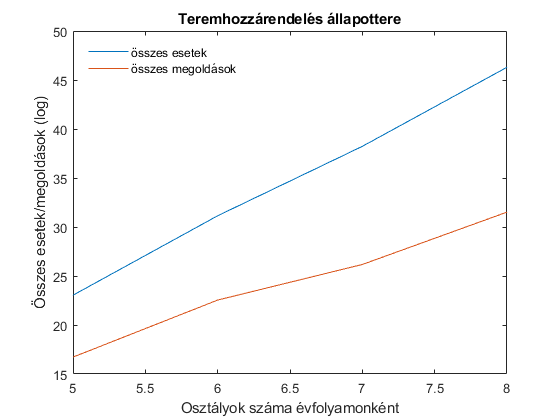
\includegraphics[width=\linewidth]{images/teremhozzarendeles.png}
\caption{Teremhozzárendelés állapottere}
\end{figure}

Az első fázis növekedési rendje a következő: $T(n,m)=\ \sim \ \Theta (2nm).$

A második fázis növekedési rendje: $T(n,m,p)=\ \sim \ \Theta (np+mp).$

Növekedési rend: $T(n,m,p)=\ \sim \ \Theta (2nm+np+mp).$

A saját példám futási idejének tudatában, a növekedési rendet felhasználva ki tudtam számolni, hogy milyen futási időre számíthatnánk a Miskolci Egyetem esetében. Az én példámban 30 terem, 30 tanár, 60 osztály, 220 osztály-tantárgy kettős és 40 időablak van, míg a Miskolci Egyetem esetében becsült adatokként 200 terem, 500 tanár, 1000 osztály, 2000 osztály-tantárgy kettős és 30 időablak. Azt kaptam, hogy $2min$ $23sec$ az átlagosan várható futási idő, a Miskolci Egyetem esetében, IntelCore i7 875K processzorral. Amely processzor 92100 műveletet végez másodpercenként.

\section{Tanárhozzárendelési feladat}

\subsection{Specifikáció}

Az osztály-tantárgy kettősökhöz immáron a tanárokat rendeljük hozzá. Ez egy halmazlefedési feladat, ami abban különbözik a halmazfelbontásitól, hogy 1:N hozzárendelés van, ugyanis egy tanárhoz több osztály-tantárgy kettőst is rendelhetünk, sőt ugye kell is többet hozzárendelni. A párosításmátrixban két feltételtől is függ, hogy 0 vagy 1 kerül a rublikába. Egyrészt, hogy az adott tanár tudja-e tanítani az adott tantárgyat, másrészt hogy az adott osztálynak van-e ilyen tárgya [3]. A minimalizálás pedig itt arra vonatkozik, hogy minél kisebb legyen a tanárok heti óraszámai közötti eltérés, ne fordulhasson elő, hogy mondjuk míg valaki 30 órát tart egy héten, addig más 5-öt.
A futtatás után kapott eredményt látva megállapítható, hogy amennyire lehetett, sikerült kiküszöbölni a tanárok egyenlőtlen terhelését, megkaptuk a lehető legoptimálisabb, olyan hozzárendelés-mátrixot, amely meghatározza, hogy egy adott osztálynak egy adott tantárgyat, melyik tanár tartsa.

\subsection{Formalizálás}

\begin{itemize}
    \item $n$: osztály-tantárgy kettősök száma
    \item $m$: tanárok száma
    \item $p$: tantárgyak száma
    \item $u \in \Bbb{N}^p$: az egyes tárgyakat hallgató osztályok száma
    \item $v \in \Bbb{N}^p$: az egyes tárgyakat oktató tanárok száma
    \item $t \in \Bbb{N}^m$: tanárok heti óraszáma
    \item $o \in \Bbb{N}^n$: osztály-tantárgy kettősök heti óraszáma
    \item $A \in \{0;1\}^{n \times m}$: párosításmátrix
    \item $X \in \{0;1\}^{n \times m}$: hozzárendelés-mátrix
\end{itemize}

\[
t_{j} =
\begin{cases}
t_j+o_i,& \hbox{ha } X_{ij}=1, \\
t_j & \hbox{egyébként}.
\end{cases}
\]

\[
A_{ij} =
\begin{cases}
1, & \hbox{ha az $i$-edik osztály-tantárgy kettősben szereplő tantárgyat tudja tanítani a $j$-edik tanár} \\
0 & \hbox{egyébként}.
\end{cases}
\]

\[
X_{ij} =
\begin{cases}
1, & \hbox{ha az $i$-edik osztály-tantárgy kettősben szereplő osztálynak az ugyanezen kettősben szereplő tantárgyat a $j$-edik tanár fogja tartani} \\
0 & \hbox{egyébként}.
\end{cases}
\]

$$\sum_{j=1}^m \vert o_jX_j-\overline{o}\vert \rightarrow \hbox{min}$$

$$\sum_{j=1}^m A_{ij} X_j=1$$

$$k=1, 2, \ldots, p$$

\subsection{Időbonyolultság}

Összes esetek száma:

$$P=m^n$$
Összes megoldások száma:

$$P=\prod_{k=1}^p v_k^{u_k}$$
A lehetséges esetek és megoldások száma (a tanárok számát plusz egy évfolyamonkénti osztály esetén 3-mal növeltem):

$$
\begin{tabular}{|l|c|c|c|c|}
\hline
& 5 & 6 & 7 & 8 \\
\hline
Összes esetek & $9,3 \cdot 10^{325}$ & $6,5 \cdot 10^{395}$ & $7,8 \cdot 10^{467}$ & $9,2 \cdot 10^{541}$ \\
\hline 
Összes megoldások & $1,1 \cdot 10^{132}$ & $2 \cdot 10^{168}$ & $4,2 \cdot 10^{208}$ & $1,2 \cdot 10^{249}$ \\
\hline
\end{tabular}
$$

\begin{figure}
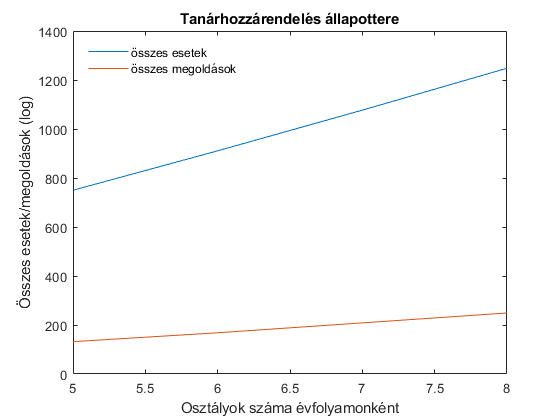
\includegraphics[width=\linewidth]{images/tanarhozzarendeles.png}
\caption{Tanárhozzárendelés állapottere}
\end{figure}

Növekedési rend: $T(n,m)=\Theta (nm+nm^2).$

A növekedési rend értelmében $4min$ $29sec$ az átlagosan várható futási idő, a Miskolci Egyetem esetében, IntelCore i7 875K processzorral. 

\section{Időablakok beosztása}

\subsection{Specifikáció}

Ennek lényege, hogy a korábbiak alapján kapott osztály-tantárgy-terem-tanár
hozzárendeléseket ütközésmentesen beosszuk időablakokba. Merthogy egy időablakban nyilván nem szerepelhet többször ugyanaz az osztály, ugyanaz a terem és ugyanaz a tanár sem. Egy időablak legfeljebb annyi hozzárendelést tartalmazhat, amennyi a tanárok száma. Amire még oda kell figyelni, hogy egy osztály-tantárgy kettős annyiszor forduljon elő, amennyi a heti óraszáma az adott osztálynak az adott tárgyból.

\subsection{Formalizálás}

\begin{itemize}
    \item $n \in \Bbb{N}$: osztály-tantárgy kettősök száma
    \item $m \in \Bbb{N}$: tanárok száma
    \item $p \in \Bbb{N}$: tantermek száma
    \item $r \in \Bbb{N}$: időablakok száma
    \item $o \in \Bbb{N}^n$: osztály-tantárgy kettősök heti óraszámai
    \item $c \in \Bbb{N}^n$: osztály-tantárgy kettősök előfordulásainak száma
    \item $e \in \Bbb{N}^m$: tanárok előfordulásainak száma
    \item $h \in \Bbb{N}^p$: tantermek előfordulásainak száma
\end{itemize}

$$\sum_{i=1}^n c_i \in (0,1), \quad \hbox{minden }l\hbox{ időablak esetén.}$$

$$\sum_{j=1}^m e_j \in (0,1), \quad \hbox{minden }l\hbox{ időablak esetén.}$$

$$\sum_{k=1}^p h_k \in (0,1), \quad \hbox{minden }l\hbox{ időablak esetén.}$$

$$\sum_{i=1}^n \vert o_i - c_i \vert = 0$$

$$l=1, 2, \ldots, r$$

\subsection{Időbonyolultság}

Összes esetek száma:

$$P=\binom{n+m-1}{m}$$
Összes megoldások száma:

$$P=\binom{n}{m}$$
A lehetséges esetek és megoldások száma (a tanárok számát plusz egy évfolyamonkénti osztály esetén 3-mal növeltem):

$$
\begin{tabular}{|l|c|c|c|c|}
\hline
& 5 & 6 & 7 & 8 \\
\hline
Összes esetek & $5 \cdot 10^{105}$ & $9,1 \cdot 10^{119}$ & $1,7 \cdot 10^{134}$ & $3,5 \cdot 10^{148}$ \\
\hline 
Összes megoldások & $8,9 \cdot 10^{36}$ & $6,8 \cdot 10^{41}$ & $4,5 \cdot 10^{46}$ & $2,7 \cdot 10^{51}$ \\
\hline
\end{tabular}
$$

\begin{figure}
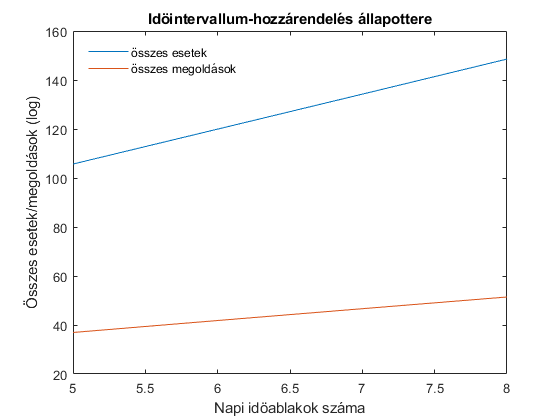
\includegraphics[width=\linewidth]{images/idoablak.png}
\caption{Időablakbeosztás állapottere}
\end{figure}

Növekedési rend: $T(n,m,r)=\ \sim \ \Theta(nmr)$.

A növekedési rend értelmében $6min$ $15sec$ az átlagosan várható futási idő, a Miskolci Egyetem esetében, IntelCore i7 875K processzorral. 

\section{Időintervallumok hozzárendelése}

A megkapott időablakok még nincsenek időintervallumhoz kötve, bármelyik felcserélhető bármelyikkel. Azt a feladatot, hogy a megadott plusz feltételek alapján lehető legoptimálisabban állapítsuk meg, mely időablak mely időintervallumba kerüljön (vagyis a legoptimálisabb legyen az időablakok sorrendje), a genetikus algoritmus végzi el nekünk.

\subsection{Probléma modellezése}

\noindent A probléma leképezése a genetikus algoritmus összetevőire:

\begin{itemize}
    \item \textbf{gén:} Egy konkrét, általános- és középiskolák esetén egy óra hosszúságú, 	          főiskolák/egyetemek esetén két óra hosszúságú időintervallum. Implementációja szótár, két elemmel: nap (enum) és a napon belüli időablak (string).
    \item \textbf{egyed:} Az összes időablak sorrendje, az egyedek mibenlétét a gének sorrendje határozza meg. Implementációja szintén szótár, elemei a gének listája, a célfüggvény-érték és az
egyedi azonosító.
    \item \textbf{populáció:} Az egyedek összességét tárolja, melyeknek számát a programozó állapítja meg, a hatékonysági tesztek által. Implementációja lista.
    \item \textbf{célfüggvény:} Esetemben a kora reggeli/késői délutáni órák számát akarom minimalizálni, illetve a napi óraszámok arányos eloszlása/pénteki órák számának minimalizálása is szempont. Minden tanárhoz tartozik egy \textsl{balance} és egy \textsl{extremisms} érték,
melyet a felhasználó ad meg és ezzel skálán rögzíti mennyire fontosak/kevésbé fontosak ezek a különböző szempontok az adott tanároknak. Ezek az értékek adják a célfüggvény súlyozását, melynek értéke ennek megfelelően minden problémás időintervallum esetén növekszik. Minél kisebb a célfüggvény értéke, az egyed annál megfelelőbb.
    \item \textbf{szelekció:} Rátermettség-arányos választással, súlyozott random generátornak köszönhetően. Miután a populáció egyedeit a célfüggvény-értékek alapján sorrendbe rakta a rendező metódusunk, a súlyozott random generátor annak megfelelő valószínűséggel szelektálja ki szülőnek az egyedeket, amilyen helyezést foglalnak el a listán. Ahány egyedből áll a populáció, a legmegfelelőbb egyednek annyiszor nagyobb esélye lesz, mint a leggyengébb egyednek. Amire még oda kell figyelni, hogy ugyanaz az egyed ne kerülhessen kétszer is kiválasztásra a szülők meghatározásakor, mivel az azt jelentené hogy a gyerek anyja egyben az apja is (igaz, a South Park rajzfilmsorozatban találkozhatunk ilyennel)...
    \item \textbf{keresztezés:} Egypontos keresztezéssel. Véletlenszám-generálással döntjük el, hol legyen a keresztezési pont. A nehézséget annak megoldása jelenti, hogy ugyanaz az időablak (vagyis ugyanaz a gén) ne fordulhasson elő többször a gyermek egyedben.
\end{itemize}

\subsection{Formalizálás}

\begin{itemize}
    \item P: populáció mérete
    \item G: generációk száma
    \item I: időablakok száma
    \item $n \in \Bbb{N}$: osztály-tantárgy kettősök száma
    \item $m \in \Bbb{N}$: tanárok száma
    \item $o \in \Bbb{N}$: osztály-tantárgy kettősök heti óraszámai
    \item $b \in \{1;5\}$: tanárok \textit{balance} értékei
    \item $e \in \{1;5\}$: tanárok \textit{extremisms} értékei
    \item $c: \Bbb{N} \rightarrow \Bbb{N}$: célfüggvény
\end{itemize}

$$ c=\sum_{j=1}^m \sum_{l=1}^I \quad
\begin{cases}
b_j, & \hbox{ha a \textit{balance}-szal kapcsolatos feltétel teljesül }l\hbox{ időablakban,}\\
e_j, & \hbox{ha a \textit{extremisms}-zel kapcsolatos feltétel teljesül }l\hbox{ időablakban,}\\
b_j+e_j, & \hbox{ha a \textit{balance}-szal és az \textit{extremisms}-zel kapcsolatos feltétel is teljesül }l\hbox{ időablakban,}\\
0 & \hbox{egyébként.}
\end{cases} 
\rightarrow min$$

\subsection{Időbonyolultság}

Összes esetek száma:

$$P=I^I$$
Összes megoldások száma:

$$P=I!$$
A számszerűsített példában itt nem évfolyamonkénti osztályok száma lesz, hanem napi időablakok száma. Az egyetemek/főiskolák kapcsán 6 (egy dupla óra egy időablak), az általános iskolák kapcsán 7, a középiskolák kapcsán pedig 8 időablakkal számolunk. Hangsúlyozom, hogy ez csak példa, a felhasználó mást is megadhat.

$$
\begin{tabular}{|l|c|c|c|}
\hline
6 & 7 & 8 \\
\hline
Összes esetek & $46656$ & $823543$ & $16777216$ \\
\hline 
Összes megoldások & $720$ & $5040$ & $40320$ \\
\hline
\end{tabular}
$$

\begin{figure}
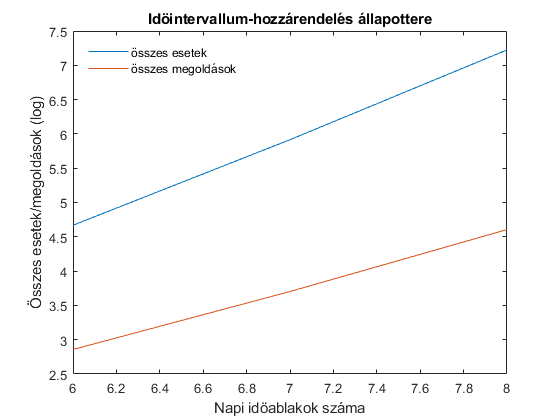
\includegraphics[width=\linewidth]{images/idointervallum.png}
\caption{Időintervallum-hozzárendelés állapottere}
\end{figure}

Célfüggvény növekedési rendje: $T(n,m,o)=\Theta(nmo)$.

Keresztezés növekedési rendje: $T(I)=\ \sim \ \Theta(I^2)$.

Hozzájön még ehhez a tiszta öröklődés, a mutáció és a rendező metódus növekedési rendje, de ezek elhanyagolhatóak. A tiszta öröklődés és a mutáció egyetlen rövid ciklusból áll, ami egy csupán 30-40 elemű listán iterál végig, a minimum rendezés növekedési rendje pedig ugyan négyzetes, de csak generációnként egyszer kerül meghívásra.

Növekedési rend: $T(P,G,I,n,m,o)=\ \sim \ \Theta(G \cdot P \cdot (nmo+I^2))$.

A tesztelés során az derült ki, hogy átlagosan 48 generációra van szükség, így a növekedési rend értelmében $48min 25sec$ az átlagosan várható futási idő, a Miskolci Egyetem esetében, IntelCore i7 875K processzorral. Ha vannak részmunkaidős tanárok és ezért vizsgáljuk, illetve büntetjük az ezzel kapcsolatos értékeket is a célfüggvényben, akkor néhány másodperccel több.

Könnyen belátható, hogy a célfüggvény és azon belül a tanárokon végigiteráló ciklus "dobja meg" a futási időt. Amennyiben nem adunk rá lehetőséget minden tanárnak, hogy a saját \textit{balance} és \textit{extremisms} értékeivel rendelkezzen, hanem egységesen állítjuk be ezeket az értékeket/alapértelmezett értékkel számolunk, akkor kevesebb mint $5 sec$ lesz a futási idő. Amennyiben adunk, az sem jelent nagy problémát, főleg ha szervergéphez méltó, az enyémtől 2x, 3x nagyobb teljesítményű processzorral rendelkezünk.

Maga a generálás (a szűkebb értelemben vett generálás) a \textit{generator.py} modul algoritmusai által történik, $11 sec$ futási ideje azonban jelentéktelen. Az én processzorommal az egész órarendgenerálási folyamat átlagosan várható futási ideje, összesen $61min$ $43sec$ tanáronkénti \textit{balance} és \textit{extremisms} értékek esetén, egységes értékek esetén pedig $13min$ $23sec$. Ha a tanárokat manuálisan akarja hozzárendelni az osztályokhoz a felhasználó, akkor még kevesebb, mivel ebben az esetben a tanárhozzárendelési feladatot nem kell végrehajtani. Kijelenthetjük, hogy nem létezik olyan méretű oktatási intézmény, melynek esetében ne tudnának belátható időn belül eredményt szolgáltatni az algoritmusaim.

\newpage

\chapter{Fejlesztői dokumentáció}

\section{Algoritmizálás}

\subsection{Osztálydefiníciók}

\begin{python}
class Room:
    def __init__(self, name, capacity, subjects):
        self.name = name
        self.capacity = capacity
        self.subjects = subjects


class Teacher:
    def __init__(self, name, subjects, balance, extremisms, begin_time,
                 end_time):
        self.name = name
        self.subjects = subjects
        self.balance = balance
        self.extremisms = extremisms
        self.begin_time = begin_time
        self.end_time = end_time


class SimpleGroup:
    def __init__(self, name, grade, subjects, headcount):
        self.name = name
        self.grade = grade
        self.subjects = []
        for subject_name, subject_data in subjects.items():
            subject = Subject(subject_name, **subject_data)
            self.subjects.append(subject)
        self.room = ""
        self.headcount = headcount


class Subject:
    def __init__(self, name, type, weekly_periods):
        self.name = name
        self.type = type
        self.weekly_periods = weekly_periods


class Group:
    def __init__(self, name, grade, subject, type, weekly_periods,
                 headcount):
        self.name = name
        self.grade = grade
        self.subject = subject
        self.type = type
        self.weekly_periods = weekly_periods
        self.room = ""
        self.teacher = ""
        self.headcount = headcount
\end{python}

Legelőször az osztálydefiníciókat láthatjuk. Mint már tudjuk, 4 tényezőnk van az órarendgenerálással kapcsolatban, viszont az osztályok kezelése kétféleképpen történik. A teremhozzárendelési feladat első fázisában még az eredeti formában (\textit{simple\_group}) kezeljük őket, utána viszont már "táblázatos" formában (\textit{group}). Hogy utóbbi mit jelent, azt korábban már kifejtettem.

\subsection{Teremhozzárendelési feladat}

\begin{python}
pairings = [[] for _ in range(len(simple_groups))]
idles = [[] for _ in range(len(simple_groups))]
for simple_group in range(len(simple_groups)):
    for room in range(len(rooms)):
        if simple_groups[simple_group].headcount <= rooms[room].capacity:
            pairings[simple_group].append(1)
            idles[simple_group].append(rooms[room].capacity -
            simple_groups[simple_group].headcount)
        else:
            pairings[simple_group].append(0)
            idles[simple_group].append(math.nan)

seated_rooms = []
seated_types = []
for simple_group in range(len(simple_groups)):
    min = math.inf
    minindex = math.nan
    type = ""
    for room in range(len(rooms)):
        ok = False
        if (pairings[simple_group][room] == 1) and\
           (idles[simple_group][room] < min):
            for seated_room in range(len(seated_rooms)):
                if (rooms[room] == seated_rooms[seated_room]) and\
                   (simple_groups[simple_group].subjects[0].type ==
                    seated_types[seated_room]):
                    ok = True
                    break
            if not ok:
                min = idles[simple_group][room]
                minindex = room
                type = simple_groups[simple_group].subjects[0].type
                simple_groups[simple_group].room = rooms[room]
        if room == len(rooms) - 1:
            seated_rooms.append(rooms[minindex])
            seated_types.append(type)
\end{python}

A teremhozzárendelési feladat első fázisa két algoritmusból áll. Az első elkészíti azt a párosításmátrixot, amely minden terem és minden osztály esetében rögzíti, hogy az adott osztály befér-e az adott terembe és ha igen, mennyi lesz a kihasználatlanság. A második algoritmus már a hozzárendeléseket végzi el a párosításmátrix eredményeit felhasználva, optimálisan, azt is figyelembe véve, hogy az egyes osztályok alaposztályok vagy nyelvi, fakutációs, egyéb osztályok. Ugyanis egy alaposztály és egy, az évfolyamon képzett nyelvi, fakultációs vagy egyéb osztály beosztható ugyanabba a terembe.

\begin{python}
def createTable(groups):
    rows = []
    for group in groups:
        for subject in group.subjects:
            row = Group(group.name, group.grade, subject.name,
                  subject.type, subject.weekly_periods, group.headcount)
            rows.append(row)
    return rows


groups = createTable(simple_groups)
for simple_group in range(len(simple_groups)):
    for group in range(len(groups)):
        if groups[group].name == simple_groups[simple_group].name:
            ok = False
            for subject in range(len(simple_groups[simple_group].
                                     room.subjects)):
                if groups[group].subject ==\
                   simple_groups[simple_group].room.subjects[subject]:
                    ok = True
                    break
            if not ok:
                ok = True
                for room in range(len(rooms)):
                    for subject in range(len(rooms[room].subjects)):
                        if groups[group].subject ==\
                           rooms[room].subjects[subject]:
                            ok = False
                            break
            counter = 0
            if not ok:
                paired = False
                while not paired and counter != 10000:
                    counter += 1
                    rand_room = rooms[random.randint(0, len(rooms) - 1)]
                    for subject in range(len(rand_room.subjects)):
                        if (groups[group].subject ==
                           rand_room.subjects[subject]) and\
                           (groups[group].headcount <= 
                           rand_room.capacity):
                            groups[group].room = rand_room.name
                            paired = True
                            break
            if ok or counter == 10000:
                groups[group].room = simple_groups[simple_group].room.name
\end{python}

A teremhozzárendelési feladat második fázisában a \textit{createTable()} metódus segítségével a \textit{simple\_group} típusú osztály objektumainkat \textit{group} típusúakká alakítjuk, majd minden osztály esetében végignézzük az összes hozzá tartozó tantárgyat. Ha találunk olyan tárgya(ka)t, mely(ek)hez van "speciális" terem/termek, de az első fázis során hozzárendelt terem nem ilyen, akkor az osztály úgymond költözni fog az adott tantárgy kapcsán (vagyis az adott osztály-tantárgy kettőshöz másik terem rendelődik hozzá). Kivéve ha nagyobb a létszámuk minden ilyen terem befogadóképességénél, ez esetben maradnak az eredetileg hozzárendelt teremben (vagyis az adott osztály-tantárgy kettőshöz ugyanazt a termet rendeljük hozzá).

\subsection{Tanárhozzárendelési feladat}

\begin{python}
pairings = [[] for _ in range(len(groups))]
for group in range(len(groups)):
    for teacher in range(len(teachers)):
        for subject in range(len(teachers[teacher].subjects)):
            if groups[group].subject ==\
               teachers[teacher].subjects[subject]:
                pairings[group].append(1)
                break
            elif subject == len(teachers[teacher].subjects) - 1:
                pairings[group].append(0)

sum_periods = [0] * len(teachers)
for group in range(len(groups)):
    for teacher in range(len(teachers)):
        if pairings[group][teacher] == 1:
            paired = True
            for other_teacher in range(teacher, len(teachers)):
                if (sum_periods[other_teacher] < 
                   sum_periods[teacher]) and\
                   (pairings[group][other_teacher] == 1):
                    paired = False
                    break
            if paired:
                groups[group].teacher = teachers[teacher].name
                sum_periods[teacher] += groups[group].weekly_periods
                break
\end{python}

Következő a tanárhozzárendelési feladat. Először itt is egy párosításmátrixot készítünk el, ami ezúttal tanárokat és osztály-tantárgy kettősöket vizsgál. Végigmegyünk a tanárok \textit{subjects} nevű, tömb típusú attribútumának elemein és ha találunk köztük olyat, ami megegyezik az adott osztály-tantárgy kettős tantárgy attribútumának értékével, akkor 1 kerül a "rublikába", ellenkező esetben 0.
A második algoritmus elvégzi a hozzárendeléseket, két dolgot vizsgálva. Az egyik a párosításmátrix értéke az adott tanár és osztály-tantárgy kettős viszonylatában, ami mindenféleképpen 1 kell, hogy legyen, a másik pedig, hogy van-e olyan másik tanár, aki szintén tudja tanítani az adott tárgyat és a heti óraszámának aktuális értéke kisebb. Ha nincs ilyen, akkor megtaláltuk azt a tanárt, akinek hozzárendelése optimális eredményre vezet az egyes tanárok terhelése közti különbségek minimalizálása kapcsán. Ez esetben hozzárendeljük őt az osztály-tantárgy kettőshöz.

\subsection{Időablakok beosztása}

\begin{python}
DAILY_PERIODS = end_time - begin_time
NUM_TIME_WINDOWS = DAILY_PERIODS * 5


def getPeriod():
    period = {'day': "", 'period': "", 'assignments': []}
    seated_groups = []
    viewed_groups = []
    for _ in range(len(teachers)):
        while True:
            if len(viewed_groups) == len(groups):
                return period
            rand = random.randint(0, len(groups) - 1)
            rand_group = groups[rand]
            ok = False
            for viewed_group in range(len(viewed_groups)):
                if rand == viewed_groups[viewed_group]:
                    ok = True
                    break
            if not ok:
                viewed_groups.append(rand)
                if sum_periods[rand] < rand_group.weekly_periods:
                    ok = True
                    for seated_group in range(len(seated_groups)):
                        if (rand_group.name ==
                           seated_groups[seated_group].name) or\
                           (rand_group.grade == 
                           seated_groups[seated_group].grade and
                           rand_group.type != 
                           seated_groups[seated_group].type):
                            ok = False
                            break
                        elif rand_group.room ==\
                           seated_groups[seated_group].room:
                            ok = False
                            break
                        elif rand_group.teacher ==\
                           seated_groups[seated_group].teacher:
                            ok = False
                            break
                    if ok:
                        seated_groups.append(rand_group)
                        sum_periods[rand] += 1
                        period['assignments'].append(rand_group)
                        break
    return period


sum_periods = [0] * len(groups)
    periods = []
    for period in range(NUM_TIME_WINDOWS):
        periods.append(getPeriod(groups, teachers, sum_periods))
\end{python}

Következő az időablakok beosztása. Itt már előre definiált konstansok is vannak. A felhasználó adja meg, hogy mettől meddig terjedjenek a napi időintervallumok, amely értékek a \textit{begin\_time} és \textit{end\_time} változókban adódnak át. Pl. ha reggel 7 és délután 4 óra között van tanítás az egyes napokon, akkor a \textit{begin\_time} 7, az \textit{end\_time} pedig 16 lesz, a \textit{DAILY\_PERIODS} konstans pedig a kettő különbségeként 9, ennyi időablak lesz egy napon. A \textit{NUM\_TIME\_WINDOWS} a heti összes időablak száma, ami így ennek ötszöröse, a \textit{MAX\_ASSIGNMENTS} által pedig azt rögzítjük, legfeljebb hány osztály-tantárgy-terem-tanár hozzárendelés lehet egy időablakban, ami a tanárok számával lesz megegyező. A lényegi részt a \textit{getPeriod()} metódus adja, ami két feltételnek eleget tevő megoldást szolgáltat. Az egyik az ütközésmentesség, vagyis hogy egy időablakban ugyanaz az osztály, ugyanaz a terem és ugyanaz a tanár sem fordulhat elő többször, sőt egy alaposztály és annak évfolyamán képzett nyelvi, fakultációs vagy egyéb osztály, illetve utóbbiak közül egyszerre több sem kerülhet ugyanabba az időablakba. A másik, hogy egy osztály-tantárgy kettősnek annyiszor kell összesen előfordulnia, amennyi a rögzített heti óraszáma az adott osztálynak az adott tárgyból. Ezt a \textit{getPeriod()} metódust aztán annyiszor hívjuk meg, amennyi a heti összes időablak száma. Az, hogy ez elegendő legyen, vagyis minden tanórának jusson időablak, a felhasználó felelőssége.

\subsection{Időintervallumok hozzárendelése genetikus algoritmussal}

\begin{python}
SIZE_POPULATION = 100
CROSSOVER_RATE = 80
MUTATION_RATE = 5
SCALE_MAX = 5
DAILY_PERIODS = end_time - begin_time
NUM_GENS = DAILY_PERIODS * 5
time_windows = {'m': [], 'tu': [], 'w': [], 'th': [], 'f': []}


class Day(Enum):
    m = 0
    tu = 1
    w = 2
    th = 3
    f = 4


for day in range(5):
    day = Day(day)
    counter = 0
    for period in range(DAILY_PERIODS):
        time_windows[day.name].append(begin_time + counter)
        counter += 1
\end{python}

Elérkeztünk az időintervallumok hozzárendeléséhez, genetikus algoritmus segítségével. Először a globális változók definiálását és a \textit{time\_windows} szótár feltöltését láthatjuk. A populáció létszámának, valamint a keresztezési és mutációs rátáknak a meghatározása tapasztalati úton történt, a \textit{SCALE\_MAX} azt rögzíti, hogy ötös skálán kell a felhasználónak megválasztani a tanárok \textit{balance} és \textit{extremisms} attribútumainak értékeit, a többi pedig már ezelőtt is előfordult. A \textit{time\_windows} szótár 5 tömböt tartalmaz, melyek a hét napjai, azok elemei pedig az időintervallumok. Azt, hogy hány eleműek ezek a tömbök és milyen időintervallumokat tartalmaznak, előzetesen nem tudni, így a lentebb található algoritmus fogja őket feltölteni, miután megvan a felhasználó által megadott \textit{begin\_time}, és az abból származtatott \textit{DAILY\_PERIODS} érték.

\begin{python}
def getRandomGens():
    gens = {'days': [], 'periods': []}
    seated_windows = {'days': [], 'periods': []}
    for gen in range(NUM_GENS):
        ok = False
        rand_day = math.nan
        rand_period = math.nan
        while not ok:
            ok = True
            rand_day = random.randint(0, 4)
            rand_day = Day(rand_day)
            rand_period =\
                time_windows[rand_day.name][random.randint(0, 
                DAILY_PERIODS - 1)]
            for seated_window in range(len(seated_windows['days'])):
                if (rand_day.name ==
                   seated_windows['days'][seated_window]) and\
                   (rand_period == 
                   seated_windows['periods'][seated_window]):
                    ok = False
                    break
        gens['days'].append(rand_day.name)
        gens['periods'].append(rand_period)
        seated_windows['days'].append(rand_day.name)
        seated_windows['periods'].append(rand_period)
    return gens
\end{python}

A \textit{getRandomGens()} metódus annyiszor megy végig ciklusban, amennyi az egyed génjeinek száma, ami a heti összes időablak száma. Minden génhez (időablakhoz) generál véletlenszerűen egy napot és egy, a napon belüli időintervallumot, nyilván ismétlődés nélkül. Ezáltal az egyedek a \textit{gens} változójukban véletlenszerű sorrendben fogják tartalmazni az időintervallumokat.

\begin{python}
def targetFunction(entity):
    diff = 0
    for period in range(NUM_GENS):
        if entity['gens']['days'][period] == "f":
            diff += balance * len(periods[period]['assignments']) * 2
        if entity['gens']['periods'][period] == time_windows['f'][0]:
            diff += (SCALE_MAX - extremisms + 1) *\
                len(periods[period]['assignments']) * 2
        elif entity['gens']['periods'][period] == time_windows['f'][1]:
            diff += (SCALE_MAX - extremisms + 1) * len(periods[period]['assignments'])
        elif entity['gens']['periods'][period] ==\
           time_windows['f'][DAILY_PERIODS - 1]:
            diff += extremisms * len(periods[period]['assignments']) * 2
        elif entity['gens']['periods'][period] ==\
           time_windows['f'][DAILY_PERIODS - 2]:
            diff += extremisms * len(periods[period]['assignments'])
    return diff
\end{python}

\begin{python}
def targetFunction(entity):
    diff = 0
    for teacher in range(len(teachers)):
        for period in range(NUM_GENS):
            for assignment in range(len(periods[period]['assignments'])):
                if periods[period]['assignments'][assignment].teacher ==\
                   teachers[teacher].name:
                    if entity['gens']['days'][period] == "f":
                        diff += teachers[teacher].balance *\
                            len(periods[period]) * 2
                    if entity['gens']['periods'][period] ==\
                       time_windows['f'][0]:
                        diff += (SCALE_MAX -
                            teachers[teacher].extremisms + 1) *\
                            len(periods[period]) * 2
                    elif entity['gens']['periods'][period] ==\
                       time_windows['f'][1]:
                        diff += (SCALE_MAX -
                            teachers[teacher].extremisms + 1) *\
                            len(periods[period])
                    elif entity['gens']['periods'][period] ==\
                       time_windows['f'][DAILY_PERIODS - 1]:
                        diff += teachers[teacher].extremisms *\
                            len(periods[period]) * 2
                    elif entity['gens']['periods'][period] ==\
                       time_windows['f'][DAILY_PERIODS - 2]:
                        diff += teachers[teacher].extremisms *\
                            len(periods[period])
    return diff
\end{python}

\begin{python}
def targetFunction(entity):
    diff = 0
    for teacher in range(len(teachers)):
        for period in range(NUM_GENS):
            for assignment in range(len(periods[period]['assignments'])):
                if periods[period]['assignments'][assignment].teacher ==\
                   teachers[teacher].name:
                    if (entity['gens']['periods'][period] < 
                       teachers[teacher].begin_time) or\
                       (entity['gens']['periods'][period] > 
                       teachers[teacher].end_time):
                        diff += SCALE_MAX * 2
                    if entity['gens']['days'][period] == "f":
                        diff += teachers[teacher].balance *\
                            len(periods[period]) * 2
                    if entity['gens']['periods'][period] ==\
                       time_windows['f'][0]:
                        diff += (SCALE_MAX - 
                            teachers[teacher].extremisms + 1) *\
                            len(periods[period]) * 2
                    elif entity['gens']['periods'][period] ==\
                       time_windows['f'][1]:
                        diff += (SCALE_MAX - 
                            teachers[teacher].extremisms + 1) *\
                            len(periods[period])
                    elif entity['gens']['periods'][period] ==\
                       time_windows['f'][DAILY_PERIODS - 1]:
                        diff += teachers[teacher].extremisms *\
                            len(periods[period]) * 2
                    elif entity['gens']['periods'][period] ==\
                       time_windows['f'][DAILY_PERIODS - 2]:
                        diff += teachers[teacher].extremisms *\
                            len(periods[period])
    return diff
\end{python}

Az, hogy a célfüggvény (\textit{targetFunction()} metódus) milyen előfordulásokat (vagy azok hiányát) "büntessen" és milyen súllyal, azt a programozó szabadon megválaszthatja, bármit bele lehet tenni. Az is megvalósítható, hogy a felhasználó eldönthesse, milyen tényezők érdeklik egyáltalán. Mint látható, 3-féle verziót készítettem. Az első verzió a kora reggeli/késő délutáni órák minimalizálását és a napi óraszámok arányos eloszlását/pénteki órák minimalizálását egységesen megadott/alapértelmezett súlyozással végzi. A másodiknál minden tanár esetén beállíthatja a felhasználó ötös skálán, milyen fontosak neki az egyes feltételek. Ezek az értékek adják ugye a súlyokat. Megemlítendő még, hogy a kora reggeli/késő délutáni órák minimalizálása kapcsán az adott napok első és második, valamint utolsó és utolsó előtti időintervallumánál is büntetőpontok járnak, az első és utolsó időintervallum esetében kétszeresen. A harmadik verzióban ezenkívül még a részmunkaidős tanárok olyan időintervallumokban való előfordulása is büntetést von maga után, amikor nem érnek rá. A futási idő egészen minimálisan lesz csak több a harmadik verzióban a másodikhoz képest, mert ugyanaz a ciklikus bonyolultság, ebből két következtetést vonhatunk le. Az egyik, hogy mivel ebben az esetben úgyis végig kell vizsgálni minden tanár előfordulását minden időintervallumban, így nyugodtan lehetnek tanáronkénti súlyok egységes helyett, a másik pedig, hogy mivel a második verzió esetében is végig kell vizsgálni, ezért nyugodtan hozzárakhatjuk a harmadik verzióban levő bővítést. Vagyis az első vagy a harmadik verziót érdemes használni. Végül még elmondhatjuk, hogy a lyukas órák számának minimalizálását a kora reggeli/késő délutáni órák számának minimalizálásával nagy mértékig elérjük, így kifejezetten erre irányuló eljárást, ami nagyon-nagyon megnövelné a futási időt, nem jó ötlet alkalmazni. A büntetőpont (\textit{diff}) aktuális értéke mindig úgy áll elő, hogy az adott időintervallumban levő osztály-tantárgy-terem-tanár hozzárendelések számát a megfelelő súllyal szorozzuk, ennyivel növeljük a büntetőpont értékét. Ha az összes időintervallumon végigmentünk az összes tanár esetében, a célfüggvény értéke előáll az adott egyed kapcsán. Ezután egy rendező metódus következik, ami a célfüggvény értékek alapján rendezi sorba az egyedeket, majd jöhet a második generáció kitenyésztése.

\begin{python}
def selectParent(either_parent):
    while True:
        rand = random.randint(0, total - 1)
        for entity in range(SIZE_POPULATION):
            for weight in range(len(weights[entity])):
                if rand == weights[entity][weight]:
                    if entities[entity]['id'] != either_parent['id']:
                        return entities[entity]
\end{python}

A szelekciót biztosító metódus (\textit{selectParent()}) már a \textit{createChildren()} metódusból fog meghívásra kerülni. Véletlenszámot generál, melynek alsó határa 0, felső határa pedig a populáció létszámának a Fibonacci-száma (\textit{total}) - 1. A súlyozott randomgenerátor által, a rangsorban betöltött pozíciók alapján előállított \textit{weights} tömböket használja fel annak meghatározására, hogy az adott véletlenszám esetén melyik egyedet kapjuk meg, mint szülőt. Ugyanez a metódus meghívódik még egyszer, hiszen két szülője van egy gyereknek, ekkor ellenőrizni kell, hogy nehogy ugyanazt az egyedet válasszuk ki újra.

\begin{python}
def createChildren(entity):
    either_parent = selectParent({'gens': {'days': [], 'periods': []}, 
                    'diff': 0, 'id': entity})
    other_parent = selectParent(either_parent)
    order_crossover = random.randint(1, 100)
    if order_crossover > (100 - CROSSOVER_RATE):
        child = crossover(either_parent, other_parent)
    else:
        child = clear_inheritance(either_parent)
    order_mutation = random.randint(1, 100)
    if order_mutation > (100 - MUTATION_RATE):
        child = mutation(child)
    child['diff'] = targetFunction(child)
    return child
\end{python}

Miután megvan, kik lesznek a szülők, annak eldöntésére, hogy tiszta örökés legyen (az egyik szülő teljes génkészletének öröklése), keresztezés és/vagy mutáció, újabb véletlenszám generálásokra van szükség. A keresztezési ráta (\textit{CROSSOVER\_RATE}) és a mutációs ráta (\textit{MUTATION\_RATE}) értéke határozza meg a különböző esetek bekövetkezésének valószínűségét, melyek mind külön metóduson keresztül kerülnek megvalósításra.

\begin{figure}
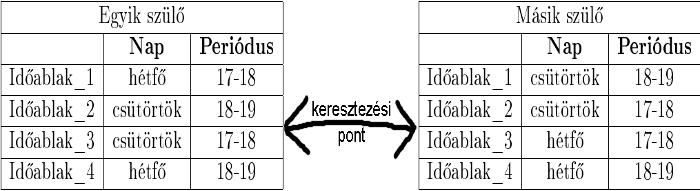
\includegraphics[width=\linewidth]{images/pelda.png}
\caption{A keresztezés problematikája}
\end{figure}

\begin{table}
\caption{Gyerek egyed}
$$
\begin{tabular}{|l|c|c|}
\hline
\multicolumn{3}{|c|}{Gyerek egyed}\\
\hline
& \bf{Nap} & \bf{Periódus}\\
\hline
Időablak\_1 & hétfő & 17-18\\
\hline
Időablak\_2 & csütörtök & 18-19\\
\hline
Időablak\_3 & hétfő & 17-18\\
\hline
Időablak\_4 & hétfő & 18-19\\
\hline
\end{tabular}
$$
\end{table}

\begin{python}
def crossover(either_parent, other_parent):
    child = {'gens': {'days': [], 'periods': []},
             'diff': 0, 'id': entity}
    crossover_point = random.randint(0, NUM_GENS - 1)
    for gen in range(0, crossover_point):
        child['gens']['days'].append(
            either_parent['gens']['days'][gen])
        child['gens']['periods'].append(
            either_parent['gens']['periods'][gen])
    for gen in range(crossover_point, NUM_GENS):
        ok = True
        for child_gen in range(len(child['gens']['days'])):
            if (child['gens']['days'][child_gen] ==
               other_parent['gens']['days'][gen]) and\
               (child['gens']['periods'][child_gen] ==
               other_parent['gens']['periods'][gen]):
                ok = False
                break
        if ok:
            child['gens']['days'].append(
                other_parent['gens']['days'][gen])
            child['gens']['periods'].append(
                other_parent['gens']['periods'][gen])
        else:
            for parent_gen in range(0, crossover_point):
                ok = True
                for child_gen in range(len(child['gens']['days'])):
                    if (other_parent['gens']['days'][parent_gen] ==
                       child['gens']['days'][child_gen]) and\
                       (other_parent['gens']['periods'][parent_gen] ==
                       child['gens']['periods'][child_gen]):
                        ok = False
                        break
                if ok:
                    child['gens']['days'].append(
                        other_parent['gens']['days'][parent_gen])
                    child['gens']['periods'].append(
                        other_parent['gens']['periods'][parent_gen])
                    break
    return child
\end{python}

A keresztező metódus (operátor) még egy utolsó véletlenszám generálást végez, ami a keresztezési pont meghatározásához szükséges. A keresztezési pont előtt levő géneket az egyik szülő génkészletéből veszi át a gyermek, az utána levőket pedig a másik szülő génkészletéből, a normál egypontos keresztezési eljárásban. Itt a képeken látható problematika miatt egy speciálisabb, bonyolultabb eljárást kellett alkotni. A probléma arról szól, hogy ha egyszerűen csak átvesszük a szülő egyedek génjeit, jó eséllyel lesz olyan időintervallum (gén), ami kétszer is elő fog fordulni a gyerek génjei között, illetve ezzel együtt olyan, amelyik egyszer sem. A keresztezési pont után jelentkezik ez a probléma és úgy küszöböljük ki, hogy amennyiben már megtalálható a gyerek génjei között a szülő adott génje, akkor a szülő keresztezési pont előtti génjei között megkeressük az első olyat, amely még nem.

\begin{python}
def clear_inheritance(either_parent):
    child = {'gens': {'days': [], 'periods': []}, 
             'diff': 0, 'id': entity}
    for gen in range(0, NUM_GENS):
        child['gens']['days'].append(either_parent['gens']['days'][gen])
        child['gens']['periods'].append(
            either_parent['gens']['periods'][gen])
    return child
\end{python}

Mint már mondtam, a tiszta öröklés esetében teljes mértékben az egyik szülő génállományát örökli a gyerek. További magyarázatot ez nem igényel.

\begin{python}
def mutation(child):
    rand_entity = entities[random.randint(0, SIZE_POPULATION - 1)]
    muted_gen = random.randint(0, NUM_GENS - 1)
    for gen in range(0, NUM_GENS - 1):
        if (child['gens']['days'][gen] ==
           rand_entity['gens']['days'][NUM_GENS - 1]) and\
           (child['gens']['periods'][gen] ==
           rand_entity['gens']['periods'][NUM_GENS - 1]):
            child['gens']['days'][gen] ==\
                child['gens']['days'][muted_gen]
            child['gens']['periods'][gen] ==\
                child['gens']['periods'][muted_gen]
            child['gens']['days'][muted_gen] ==\
                rand_entity['gens']['days'][NUM_GENS - 1]
            child['gens']['periods'][muted_gen] ==\
                rand_entity['gens']['periods'][NUM_GENS - 1]
            break
    return child
\end{python}

A mutációs metódusban (operátorban) random generálunk egy mutálandó gént és egy idegen egyedet (vagyis olyan egyedet, aki nem szülője a gyereknek). Az idegen egyed sorrendileg utolsó génjének megfelelő gént megkeressük a gyerek génjei között, és azt felcseréljük a mutálandó génnel.

\begin{python}
while True:
    new_entities = []
    for entity in range(SIZE_POPULATION):
        new_entities.append(createChildren(entity))
    entities = new_entities
    sortEntities()
    if entities[0]['diff'] - entities[SIZE_POPULATION - 1]['diff'] == 0:
        break

for gen in range(NUM_GENS):
    periods[gen]['day'] = entities[0]['gens']['days'][gen]
    periods[gen]['period'] = entities[0]['gens']['periods'][gen]
\end{python}

A generációk száma előre nem meghatározott, mert a tesztelés során kiderült, hogy az egyedek célfüggvény értékei konvergálnak az optimumhoz (a minimális értékhez) és nem csak a legjobb egyed éri el, hanem mind. Ebből kifolyólag olyan feltételhez kötöttem a leállást, hogy a legjobb egyed célfüggvény értékének meg kell egyeznie a legrosszabb egyed célfüggvény értékével. Vagyis az összes egyed célfüggvény értékének megegyezőnek kell lenni. Végül beleírjuk a \textit{periods} listába a napokat és időintervallumokat, amire a \textit{generator.py}-nak szüksége lesz.

\section{Adatbázis}

\begin{figure}
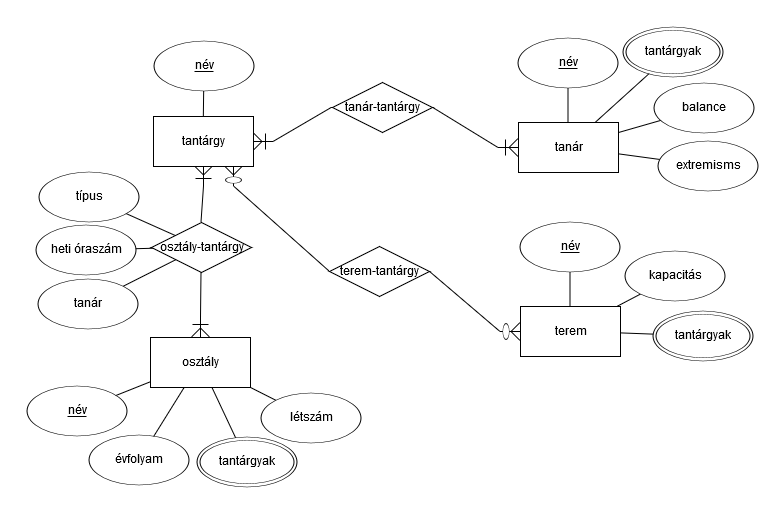
\includegraphics[width=\linewidth]{images/ermodell.png}
\caption{Az ER modell}
\end{figure}

\begin{figure}
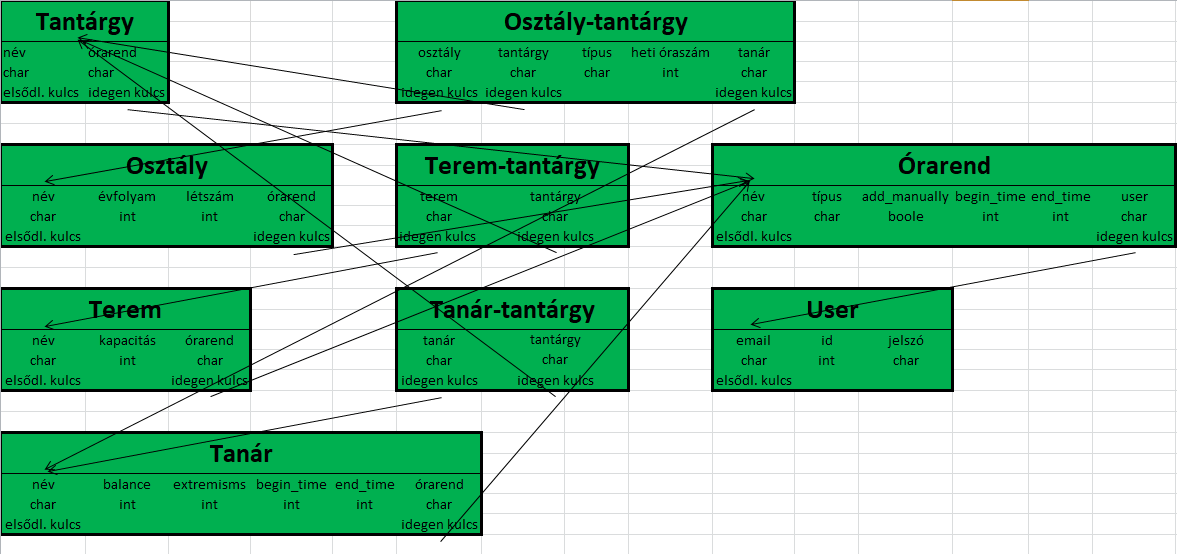
\includegraphics[width=\linewidth]{images/relmodell.png}
\caption{A relációs modell}
\end{figure}

Adatbázist kellett használni a felhasználók által létrehozott órarendek adatainak a letárolásához és felhozásához. 6 entitásunk van (osztály, tantárgy, terem, tanár, órarend, felhasználó), de a több-több kapcsolatok miatt további táblákat is létre kellett hozni, a relációs modell már tartalmazza ezeket. 1:N kapcsolat van az osztály-tantárgy kapcsolótábla és a tanár tábla között, az órarend tábla és az osztály, tantárgy, tanár, terem táblák között, valamint az órarend és felhasználó tábla közt, a többi kapcsolat N:M (osztály-tantárgy, terem-tantárgy, tanár-tantárgy). A terem-tantárgy kapcsolatok opcionálisak, mert nem muszáj tantárgynak tartoznia egy adott teremhez, ahogyan egy adott tantárgyhoz sem muszáj, hogy tartozzon terem, a többi kapcsolat kötelező. A felhasználókat leszámítva minden entitás esetén a név szolgál egyedi azonosítóként, ami egyedül a tanárok esetén okozhatna problémát, de felhívjuk rá a felhasználó figyelmét, hogy azonos nevű tanárok esetén római számokkal való megkülönböztetést használjon, ezt elkerülendő. Python-ban az adatbázis tábláit osztályokként definiáljuk, ennek kapcsán kell még egy magyarázatot megtennem. Az osztály-tantárgy kapcsolótábla tanár idegen kulcsának értéke alapértelmezetten üres string. Ennek oka, hogy a felhasználó új órarend létrehozásakor eldöntheti, maunálisan akarja-e majd hozzárendelni az osztály-tantárgy kettősökhöz a tanárokat, amennyiben nem, akkor is léteznie kell ennek az attribútumnak, de addig üres string marad az értéke, amíg a tanárhozzárendelési algoritmus során kapott eredmények nem tárolódnak az adatbázisban, és a felhasználó által közvetlenül nem megváltoztatható.

\section{Webalkalmazás}

Az egyoldalas webalkalmazás komponenseit vue fájlok alkotják, bennük egy html kódrésszel és egy script kódrésszel, amihez a Vue axios csomagját importáltam. A szkriptekben definiáltam az objektumokat (osztályok, tantárgyak, tantermek, tanárok és még többet is) a megfelelő adattagokkal és azokkal a metódusokkal, amelyek HTTP kéréseket intéznek a szerverhez (így közvetetten interakciót folytatnak az adatbázissal), illetve kliensoldali ellenőrzést végeznek. Ez utóbbira és a felhasználó által aktuálisan hozzáadott objektum példányok letárolására, illetve törlésre általam definiált metódust használtam, korábban eltárolt adatok felhozásához (bármely, de nem befoglaló objektum kapcsán) pedig a gyári \textit{created()} és \textit{mounted()} metódusokat definiáltam felül. Előbbi a komponens betöltésekor hívódik meg, utóbbi minden frissítéskor. A html kódrészben a Vue által biztosított módokon átadjuk az adatokat a megfelelő metódusnak (ezáltal "felvisszük" őket), vagy fogadjuk az adatokat a megfelelő metódustól és megjelenítjük.

A \textit{model.py} fájlban (ez egy Python modul) található az adatbázis tartalmának leképezése objektum-orientáltan, a \textit{timetable.py} HTTP kéréseket teljesítő metódusai ennek alapján tudnak az adatokra hivatkozni. Ezek a létrehozó, lekérdező, módosító, törlő metódusok mindig "ülést nyitnak", vagyis database session-t a \textit{database\_session.py} modul közbenjárásával, az adatbázishoz való hozzáféréshez. Ezenkívül egyes metódusok az adatok szerveroldali ellenőrzésére megírt metódust is meghívnak, melyeket szintén ebben a modulban definiáltam. A \textit{server.py} modulhoz futnak be a HTTP kérések a vue komponensekből, ugyanis ez a szerver. Ez a modul végzi el minden kérésnél az authentikációt, vagyis a felhasználói jogosultság ellenőrzését a token alapján, majd hívja meg a \textit{timetable.py} megfelelő metódusát, és a kapott eredményt vagy hibaértesítést aztán a HTTP protokoll szabványos formájában továbbítja a vue komponensnek. Itt használjuk fel a Falcon, a Waitress és a JWT nyújtotta szolgáltatásokat, melyeket röviden kifejtettem korábban.

Amikor a felhasználó már minden adatot felvitt és szeretné generáltatni az órarendeket, akkor a HTTP kérelem után, a \textit{server.py}-ból az adott órarendhez tartozó összes osztály, tantárgy, tanár, tanterem felhozásra kerül az adatbázisból, és ezúttal nem adjuk vissza a vue komponensnek json-ben, hanem eredeti formátumban a \textit{generator.py} számára továbbítjuk őket. A \textit{generator.py} először objektumokat példányosít a beérkezett szótár típusú adatokból, majd ezeket paraméterként átadja az órarendgenerálási részfeladatokat elvégző modulok globális metódusainak. Utána összegyűjti az adott osztályokhoz, tanárokhoz, illetve tantermekhez tartozó hozzárendeléseket, majd rendezi őket, úgy hogy a hétfői nap legkorábbi időintervalluma legyen a lista első és a pénteki nap legutolsó időintervalluma az utolsó eleme. Legvégül átadja az eredményeket az \textit{exporter.py}-nak. Az \textit{exporter.py} felelős a fájlok létrejöttéért és tartalommal való feltöltéséért. Utóbbit a Jinja segítségével valósítja meg, amely segít az eredmények html fájlokba való beleírásában. Ehhez egy \textit{template.html} nevű sablont készítettem, ami alapján a megadott helyekre a különböző osztályok, tanárok, tantermek kapcsán aktuális adatok fognak íródni. Végül Pandoc segítségével a html-eket pdf-ekké konvertáljuk.

\begin{figure}
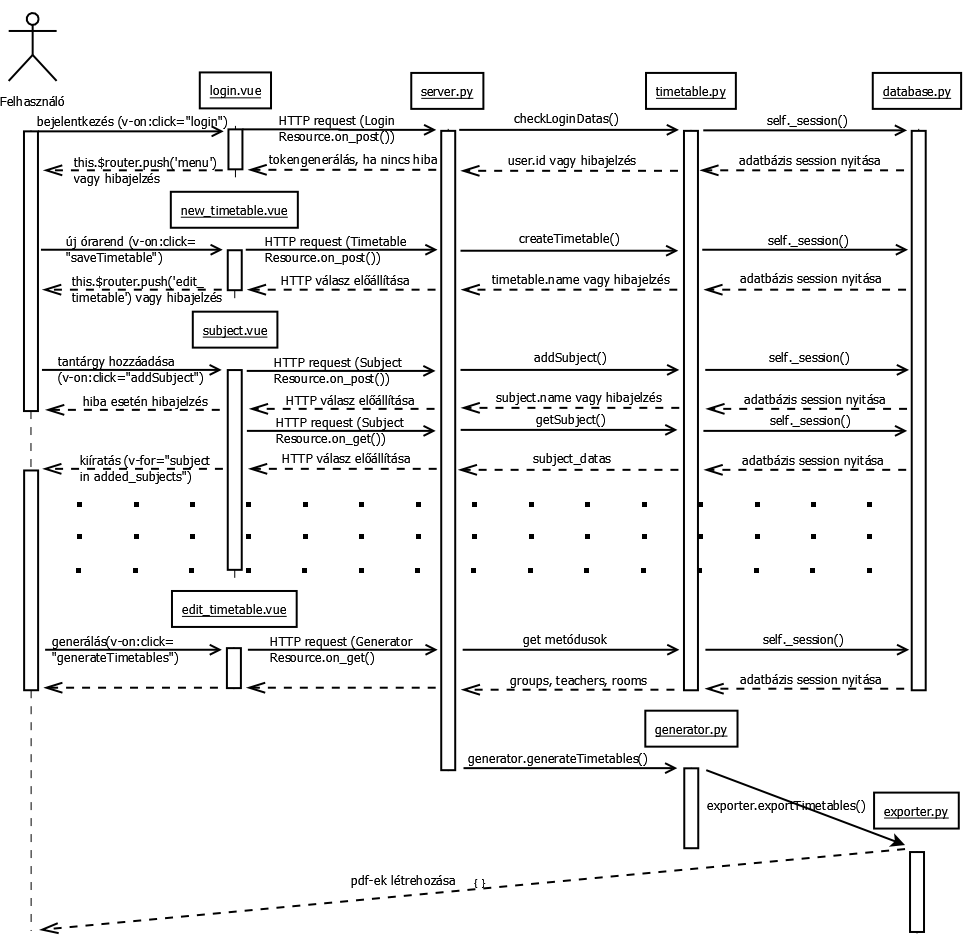
\includegraphics[width=\linewidth]{images/szekvencia.png}
\caption{Az alkalmazás szekvenciadiagramja}
\end{figure}

\section{Felhasználói dokumentáció}

A főoldal a \textit{login}, ahol bejelentkezésre van lehetőség, vagypedig ha még nem regisztráltunk vagy elfelejtettük a jelszavunkat, elérhetőek itt linkek, melyek az ezzel kapcsolatos oldalra irányítanak. Bejelentkezés után a menüben találjuk magunkat, ahol a fontos és egyben magyarázatra szoruló menüpontok, az Új órarend létrehozása és az Órarendjeim. Ha újat hozunk létre, meg kell adni a típust, hogy manuálisan akarjuk-e a tanárokat hozzárendelni az osztályokhoz, illetve hogy hány órától legyen a legkorábbi napi időablak és hány órakor érjen véget a legkésőbbi. Ezt a napi időintervallumot lesz lehetőség még szűkíteni a részmunkaidős tanárok esetében, az azonos nevű attribútumok állításával, tanár hozzáadásakor. A típus esetében általános iskola, középiskola és főiskola/egyetem közül választhatunk, ennek egyik jelentősége, hogy milyen típusú tantárgyakat lehet majd hozzáadni (pl. fakt típusú órák csak középiskolában vannak, elméletek és gyakorlatok pedig csak a főiskolán/egyetemen), a másik, hogy a főiskolán/egyetemen két óra hosszú egy időablak. Ha meglevő órarendet szeretnénk szerkeszteni, akkor kiválasztjuk melyiket szeretnénk és az abban a sorban található ceruza ikonra kattintunk (amennyiben törölni szeretnénk, akkor pedig nyilván a keresztre). Négy link fog megjelenni a számunkra, akkor is ha új órarendet hoztunk létre, akkor is ha meglevőt szerkesztünk. Egy a tantárgyak, egy a tantermek, egy a tanárok és egy az osztályok létrehozására. Új órarend esetén először mindenképpen tantárgyat/tantárgyakat kell hozzáadni, mert azzal kapcsolatban, hogy milyen tárgyai legyenek egy osztálynak, egy tanárnak, vagy hogy milyen tárgy(ak)ra legyen esetleg specializálódva egy terem, a korábban hozzáadottak közül választhatunk lenyíló listában. Ugyanígy, ha manuálisan rendeljük hozzá a tanárokat az osztályokhoz, csak a korábban hozzáadott tanárok közül választhatunk. Bármit is akarunk hozzáadni, egyszerre mindig egy példányt tudunk felvinni a megfelelő mezők kitöltésével (melyek elsősorban szövegmezők és lenyíló listák lesznek) és a hozzáadásra fenntartott nyomógomb lenyomásával. (Ez vonatkozik az osztály tantárgyainak hozzáadására is, osztály hozzáadásán belül.) Amint ez megtörtént, letárolódik az adatbázisban az adott objektum példány és a képernyő alján kiírásra is kerülnek a hozzáadott adatok, egyidejűleg alaphelyzetbe állnak a kitöltendő mezők és máris jöhet következő példány hozzáadása, ha szeretnénk. Mindez aszinkron, az oldal újratöltése nélkül történik. Ezenkívül van lehetőség törlésre, minden hozzáadott példánnyal kapcsolatban, a törlés ikonnal. Ha végeztünk a hozzáadásokkal és szeretnénk órarendet generáltatni, a Get it! gombra kell kattintani az \textit{edit\_timetable} oldalon. A felvitt adathalmaz méretétől függően sok időt is igénybe vehet az órarendgenerálás, de létre fog jönni az összes órarend pdf-jét tartalmazó mappa a fájlrendszer megadott helyén (ha publikussá tenném a webalkalmazást, akkor pedig letölthetővé válna az adott gép számára). Minden osztályé, minden tanáré és minden tanteremé külön pdf fájlban kap helyet, táblázatos formában. Bármikor van lehetőség újra generáltatni, akár ugyanazzal az adathalmazzal is. A véletlenszám-generálás miatt nem determinisztikus a folyamat, így változatlan adathalmaz esetén sem ugyanazokat a megoldásokat kapjuk újból, ha éppen nem elégedett az eredménnyel a felhasználó, próbálkozhat többször is. A \textit{my\_timetables} oldalról elérhetőek a meglevő adathalmazaink, a megfelelőt kiválasztva, a szerkesztés ikonra kattintva megintcsak az \textit{edit\_timetable} oldalon találhatjuk magunkat.

\section{Tesztelés}

A szakdolgozat készítése során folyamatosan tesztelni kellett, azt lehet mondani, hogy a tesztelések a korábbi szakaszban az órarendgeneráló algoritmusokkal kapcsolatos tesztek voltak, a későbbi szakaszban pedig a webes működésekkel kapcsolatos tesztek. Az alábbiakban konkrétan megnevezem, milyen kritikus tényezőkre kellett különösen odafigyelni, illetve hol követtem el hibát.

Teremhozzárendelési feladat:
\begin{itemize}
\item minden osztályhoz sikerült-e termet hozzárendelni
\item speciális termet igénylő tárgyak esetén, más terem van-e az osztály-tantárgy kettősökhöz hozzárendelve, mint az osztályokhoz "alapból"
\item egyes esetekben nem fér be tantárgy-specifikus terembe az osztály-tantárgy kettős, ilyenkor maradnia kell az osztálynak az alapból hozzárendelt teremben, mert valahol lenniük kell
\end{itemize}

Az időablakbeosztási feladat kapcsán biztosítani kellett, hogy amennyiben még van hely egy adott időablakban, de nincs több olyan osztály-tantárgy-terem-tanár hozzárendelés, amelyet  beoszthatnánk, akkor annak ellenére, hogy nem teljesen kitöltött az időablak, átlépjünk a következőbe. Ilyenkor keletkezhetnek lyukas órák, de ez elkerülhetetlen.

Genetikus algoritmus (időintervallum-hozzárendelési feladat):
\begin{itemize}
\item a célfüggvényben megvizsgáltuk-e a tanárok előfordulásait az egyes időablakokban, vagy elkövettük azt a hibát, hogy csak az időablakok hossza (az időablakokban levő hozzárendelések száma) alapján számoltunk
\item sikerült-e kiküszöbölni a korábban bemutatott keresztezési problematikát
\item nem adtuk-e hozzá az új egyedeket a populációs listához, mielőtt a generáció összes egyedét kitenyésztettük, ugyanis ideiglenesen egy másik listában kell letárolni őket, mert az adott generációban született egyed még nem lehet szülő
\end{itemize}

Webes működések:
\begin{itemize}
\item bejelentkezési ellenőrzésnél ne a jelszó eredeti formája és a hexadecimális kóddá konvertált kerüljön egymással összehasonlításra
\item a hitelesítésekhez használt token benne maradt-e a HTTP kérelmekben
\item lementődtek-e az adatbázisban a felvitt adatok, máskülönben esélytelen felhozni őket
\item a több-több kapcsolatok megfelelően tárolódtak-e le, különös tekintettel az osztály-tantárgy kapcsolatokra, ahol a kapcsolótáblához kötődő attribútumok is vannak
\item ha csak adott példányt vagy adott feltételnek eleget tevő példányokat akarunk felhozni,  rendben történik-e a paraméterátadás
\item csak az adott órarenden belüli tantárgyak, tantermek, tanárok és osztályok kerülnek-e felhozásra, illetve csak az adott felhasználó órarendjei vannak-e meg
\item a \textit{template.html} sablon megfelelő-e, különben nem fogja a kívánt tartalommal vagy egyáltalán tartalommal feltölteni a Jinja a html-eket
\end{itemize}

\newpage

\chapter{Összefoglalás}

Az eltervezetteknek megfelelően implementáltam azokat az algoritmusokat, amelyek végül minden feltételt kielégítő órarendeket eredményeztek. Az ezek során szerzett tapasztalatokat ugyanúgy kifejtettem a szakdolgozatban, mint ahogyan elméleti elemzést is lefolytattam, ezáltal kézzelfogható eredményeket szolgáltatva a témakörben, melyek a későbbiekben nagyban felhasználhatóak lehetnek. A vizsgálatok egyik célpontja a genetikus algoritmus volt, ennek kapcsán kijelenthetem, hogy a genetikus algoritmust az időintervallum-hozzárendelések kapcsán érdemes használni, a többi részfeladat hagyományos alogritmusokkal való megoldását követően. A szakdolgozat elején számba vett, ismert órarendgeneráló alkalmazásokhoz képest az általam készített alkalmazás többet ad, a kora reggeli/késő délutáni órák számának minimalizálásával és a napi óraszámok arányos eloszlása/pénteki órák számának minimalizálásával, miközben egyben jó hatékonyságot érhetünk el a lyukas órák számának minimalizálása kapcsán is.

\newpage

\huge{Summary}

By right of the plan, I have implemented those algorithms, which resulted timetables finally, what satisfy every conditions. Experiences, what I gained during this, I have stated in the thesis, how I have conducted theoretical analysis too, so provided the profession with handable results, which can be usable in the future in large. Genetic algorithm was either target of investigations, about it I can assert, that usage of genetic algorithm is deserved at assignments of time intervals, after we solved the other subtasks by traditional algorithms. Compare to those famous timetable generator applications, which are presented in the beginning of thesis, the application is prepared by me add us more, with minimalization of number of early morning/late afternoon periods and with harmonic distribution of daily period numbers/minimalization of friday periods, while at the same time, we can reach good effectivity about minimalization of number of holes in periods, also.

\newpage

\clearpage

\addcontentsline{toc}{chapter}{Irodalomjegyzék}
\bibliographystyle{plain}
\bibliography{styles/dolgozat.bib}

\huge{Irodalomjegyzék}

\noindent [1]\quad $Pásztor E. - Obrony B.: Ökológia. Nemzeti Tankönyvkiadó Zrt., Budapest, 2007.$

\noindent [2]\quad $Futó I.: Mesterséges intelligencia. Aula Kiadó, Budapest, 1999.$

\noindent [3]\quad $Nagy T.: Operációkutatás. Miskolci Egyetemi Kiadó, Miskolc, 1998.$

\textbf{Internetes források}

\noindent [4]\quad $https://www.timetabler.com$

\noindent [5]\quad $https://www.schedulebuilder.org$

\noindent [6]\quad $https://www.primetimetable.com$

\noindent [7]\quad $https://www.asctimetables.com$

\noindent [8]\quad $https://www.github.com$

\newpage

\pagestyle{empty}

\noindent \textbf{\Large Adathordozó használati útmutató}

\vskip 1cm

Az adathordozón megtalálható először is maga a szakdolgozat, pdf és tex fájlban is. Ezenkívül van egy \textit{styles} mappa, ami a tex fájlhoz kapcsolódó csomagokat tartalmazza, egy \textit{images} mappa a szakdolgozat képeivel, és egy \textit{application} mappa. Ez utóbbiban van az alkalmazás és minden, ami a működtetéséhez szükséges. Két fő részből, ezáltal mappából áll, mivel van a kliens oldal és a szerver oldal.

A kliensben a \textit{package.json} tartja számon a függőségeket, amiről a Felhasznált szoftverek alfejezetben beszéltem. Egyoldalas alkalmazásról beszélhetünk, melynek egységes header-jét az \textit{index.html} fájl tartalmazza, az üres body blokkba pedig az \textit{id} segítségével betöltődik az éppen aktuális vue fájl tartalma. Az \textit{src} mappában a következők találhatók:

\begin{itemize} 
\item \textit{app.vue}: ez a fájl gondoskodik róla, hogy a különböző vue fájlok (komponensek) felcímkéződjenek a html fájlba való betöltéshez szükséges \textit{id}-val
\item \textit{main.js}: ez a JavaScript fájl egy Vue objektumot példányosít, ezáltal fogjuk össze a vue komponenseinket
\item \textit{router} mappa: ebben található az \textit{index.js} router (útvonalválasztó) fájl, ami tartalmazza a különböző vue komponensek beazonosításához, eléréséhez szükséges információkat
\item \textit{components} mappa: a vue komponenseket tartalmazza, melyek funkcionálisan egy-egy html oldalnak feleltethetők meg és betöltésre várnak a webalkalmazás használata során
\end{itemize}

A szerver oldal Python fájlokat, valamint Python fájlokat tartalmazó mappákat tartalmaz. A \textit{timetable} mappában a \textit{timetable.py}, \textit{model.py} és \textit{database\_session.py} modulok vannak, az \textit{exercises} mappában pedig az órarendgeneráló algoritmusokat tartalmazó modulok, részfeladatonként egy, illetve külön mappában (\textit{classes}) az osztálydefiníciók.

Mivel az alkalmazást kipróbálni szándékozó felhasználónak is a saját gépén szükséges szervert létrehoznia, telepíteni kellhet több dolgot:
\begin{itemize}
\item \textit{npm}
\item \textit{MySQL}
\item \textit{PyCharm}
\item \textit{Python kiegészítők:}
\begin{itemize}
	\item \textit{Falcon}
	\item \textit{Waitress}
	\item \textit{JWT}
	\item \textit{Jinja}
	\item \textit{SQLAlchemy}
\end{itemize}
\end{itemize}

Ha mindez megvan, regisztráció helyett javaslom a molnarfi93@gmail.com e-mail címmel és 666 jelszóval való belépést. Ebben az esetben ugyanis, a \textit{my\_timetables} komponensből elérhető lesz az általam felvitt órarend-adathalmaz, rögtön lehet generáltatni.

\end{document}